%%%%%%%%%%%%%%%%%%%%%%%%%%%%%%%%%%%%%%%%%
% Wenneker Article
% LaTeX Template
% Version 2.0 (28/2/17)
%
% This template was downloaded from:
% http://www.LaTeXTemplates.com
%
% Authors:
% Vel (vel@LaTeXTemplates.com)
% Frits Wenneker
%
% License:
% CC BY-NC-SA 3.0 (http://creativecommons.org/licenses/by-nc-sa/3.0/)
%
%%%%%%%%%%%%%%%%%%%%%%%%%%%%%%%%%%%%%%%%%

%----------------------------------------------------------------------------------------
%	PACKAGES AND OTHER DOCUMENT CONFIGURATIONS
%----------------------------------------------------------------------------------------

\documentclass[11pt, a4paper]{article} % 10pt font size (11 and 12 also possible), A4 paper (letterpaper for US letter) and two column layout (remove for one column)

\usepackage[english]{babel} % English language hyphenation
\usepackage{microtype} % Better typography
\usepackage{amsmath,amsfonts,amsthm} % Math packages for equations
\usepackage[svgnames]{xcolor,colortbl} % Enabling colors by their 'svgnames'
\usepackage[hang, small, labelfont=bf, up, textfont=it]{caption} % Custom captions under/above tables and figures
\usepackage{booktabs} % Horizontal rules in tables
\usepackage{lastpage} % Used to determine the number of pages in the document (for "Page X of Total")
\usepackage{graphicx} % Required for adding images
\usepackage{amssymb}
\usepackage[mathscr]{eucal}
\usepackage[table]{xcolor}
\usepackage{enumitem} % Required for customising lists
\setlist{noitemsep} % Remove spacing between bullet/numbered list elements
\usepackage{sectsty} % Enables custom section titles
\allsectionsfont{\usefont{OT1}{phv}{b}{n}} % Change the font of all section commands (Helvetica)
\usepackage{hyperref}
\usepackage[sort,numbers]{natbib}
\usepackage{fancyhdr}
\usepackage{url}
\usepackage{floatrow}

\definecolor{Gray}{gray}{0.85}
\definecolor{LightCyan}{rgb}{0.88,1,1}
\definecolor{LightPink}{rgb}{0.25,0.5,1}
\definecolor{bubblegum}{rgb}{0.99, 0.76, 0.8}
\definecolor{pastelpink}{rgb}{1.0, 0.82, 0.86}
\definecolor{piggypink}{rgb}{0.99, 0.87, 0.85}
\definecolor{pink}{rgb}{1, 0.5, 0.9}
\definecolor{lightpink}{rgb}{1.0, 0.61, 0.76}

% ----------------------------------------------------------------------------------------
%	MARGINS AND SPACING
%----------------------------------------------------------------------------------------
\usepackage{geometry} % Required for adjusting page dimensions
\geometry{
	top=1.5cm, % Top margin
	bottom=1.5cm, % Bottom margin
	left=1.5cm, % Left margin
	right=1.5cm, % Right margin
	includehead, % Include space for a header
	includefoot, % Include space for a footer
	%showframe, % Uncomment to show how the type block is set on the page
}
\setlength{\columnsep}{6mm} % Column separation width

%----------------------------------------------------------------------------------------
%	FONTS
%----------------------------------------------------------------------------------------

\usepackage[T1]{fontenc} % Output font encoding for international characters
\usepackage[utf8]{inputenc} % Required for inputting international characters
\usepackage{XCharter} % Use the XCharter font
\usepackage{verbatim} 
%\usepackage{fontspec}
%\setmainfont{TeX Gyre Termes}
\pagestyle{headings}
\usepackage{fancyhdr}
\setlength{\headheight}{15.2pt}
\pagestyle{fancy}
%%%%%%%%%%%%%%%%%%%%%%%%%%%%%%%%%%%%%%%%%%
% Wenneker Article
% Structure Specification File
% Version 1.0 (28/2/17)
%
% This file originates from:
% http://www.LaTeXTemplates.com
%
% Authors:
% Frits Wenneker
% Vel (vel@LaTeXTemplates.com)
%
% License:
% CC BY-NC-SA 3.0 (http://creativecommons.org/licenses/by-nc-sa/3.0/)
%
%%%%%%%%%%%%%%%%%%%%%%%%%%%%%%%%%%%%%%%%%

%----------------------------------------------------------------------------------------
%	PACKAGES AND OTHER DOCUMENT CONFIGURATIONS
%----------------------------------------------------------------------------------------

\usepackage[english]{babel} % English language hyphenation

\usepackage{microtype} % Better typography

\usepackage{amsmath,amsfonts,amsthm} % Math packages for equations

\usepackage[svgnames]{xcolor} % Enabling colors by their 'svgnames'

\usepackage[hang, small, labelfont=bf, up, textfont=it]{caption} % Custom captions under/above tables and figures

\usepackage{booktabs} % Horizontal rules in tables

\usepackage{lastpage} % Used to determine the number of pages in the document (for "Page X of Total")

\usepackage{graphicx} % Required for adding images

\usepackage{enumitem} % Required for customising lists
\setlist{noitemsep} % Remove spacing between bullet/numbered list elements

\usepackage{sectsty} % Enables custom section titles
\allsectionsfont{\usefont{OT1}{phv}{b}{n}} % Change the font of all section commands (Helvetica)

%----------------------------------------------------------------------------------------
%	MARGINS AND SPACING
%----------------------------------------------------------------------------------------

\usepackage{geometry} % Required for adjusting page dimensions

\geometry{
	top=1cm, % Top margin
	bottom=1.5cm, % Bottom margin
	left=2cm, % Left margin
	right=2cm, % Right margin
	includehead, % Include space for a header
	includefoot, % Include space for a footer
	%showframe, % Uncomment to show how the type block is set on the page
}

\setlength{\columnsep}{7mm} % Column separation width

%----------------------------------------------------------------------------------------
%	FONTS
%----------------------------------------------------------------------------------------

\usepackage[T1]{fontenc} % Output font encoding for international characters
\usepackage[utf8]{inputenc} % Required for inputting international characters

\usepackage{XCharter} % Use the XCharter font

%----------------------------------------------------------------------------------------
%	HEADERS AND FOOTERS
%----------------------------------------------------------------------------------------

\usepackage{fancyhdr} % Needed to define custom headers/footers
\pagestyle{fancy} % Enables the custom headers/footers

\renewcommand{\headrulewidth}{0.0pt} % No header rule
\renewcommand{\footrulewidth}{0.4pt} % Thin footer rule

\renewcommand{\sectionmark}[1]{\markboth{#1}{}} % Removes the section number from the header when \leftmark is used

%\nouppercase\leftmark % Add this to one of the lines below if you want a section title in the header/footer

% Headers
\lhead{} % Left header
\chead{\textit{\thetitle}} % Center header - currently printing the article title
\rhead{} % Right header

% Footers
\lfoot{} % Left footer
\cfoot{} % Center footer
\rfoot{\footnotesize Page \thepage\ of \pageref{LastPage}} % Right footer, "Page 1 of 2"

\fancypagestyle{firstpage}{ % Page style for the first page with the title
	\fancyhf{}
	\renewcommand{\footrulewidth}{0pt} % Suppress footer rule
}

%----------------------------------------------------------------------------------------
%	TITLE SECTION
%----------------------------------------------------------------------------------------

\newcommand{\authorstyle}[1]{{\large\usefont{OT1}{phv}{b}{n}\color{DarkRed}#1}} % Authors style (Helvetica)

\newcommand{\institution}[1]{{\footnotesize\usefont{OT1}{phv}{m}{sl}\color{Black}#1}} % Institutions style (Helvetica)

\usepackage{titling} % Allows custom title configuration

\newcommand{\HorRule}{\color{DarkGoldenrod}\rule{\linewidth}{1pt}} % Defines the gold horizontal rule around the title

\pretitle{
	\vspace{-30pt} % Move the entire title section up
	\HorRule\vspace{10pt} % Horizontal rule before the title
	\fontsize{32}{36}\usefont{OT1}{phv}{b}{n}\selectfont % Helvetica
	\color{DarkRed} % Text colour for the title and author(s)
}

\posttitle{\par\vskip 15pt} % Whitespace under the title

\preauthor{} % Anything that will appear before \author is printed

\postauthor{ % Anything that will appear after \author is printed
	\vspace{10pt} % Space before the rule
	\par\HorRule % Horizontal rule after the title
	\vspace{20pt} % Space after the title section
}

%----------------------------------------------------------------------------------------
%	ABSTRACT
%----------------------------------------------------------------------------------------

\usepackage{lettrine} % Package to accentuate the first letter of the text (lettrine)
\usepackage{fix-cm}	% Fixes the height of the lettrine

\newcommand{\initial}[1]{ % Defines the command and style for the lettrine
	\lettrine[lines=3,findent=4pt,nindent=0pt]{% Lettrine takes up 3 lines, the text to the right of it is indented 4pt and further indenting of lines 2+ is stopped
		\color{DarkGoldenrod}% Lettrine colour
		{#1}% The letter
	}{}%
}

\usepackage{xstring} % Required for string manipulation

\newcommand{\lettrineabstract}[1]{
	\StrLeft{#1}{1}[\firstletter] % Capture the first letter of the abstract for the lettrine
	\initial{\firstletter}\textbf{\StrGobbleLeft{#1}{1}} % Print the abstract with the first letter as a lettrine and the rest in bold
}

%----------------------------------------------------------------------------------------
%	BIBLIOGRAPHY
%----------------------------------------------------------------------------------------

\usepackage[backend=bibtex,style=authoryear,natbib=true]{biblatex} % Use the bibtex backend with the authoryear citation style (which resembles APA)

\addbibresource{example.bib} % The filename of the bibliography

\usepackage[autostyle=true]{csquotes} % Required to generate language-dependent quotes in the bibliography
 % Specifies the document structure and loads requires packages
\fancyhf{}
%\fancyhead[LE,RO]{Overleaf}
%\fancyhead[RE,LO]{Guides and tutorials}
%\fancyfoot[LO,RE]{FETOPEN-01 template WP18-20 v20171106}
\fancyfoot[LE,RO]{$\mathcal{ROBHOOT}$}
%\fancyfoot[LE,RE]{\thepage} % pa
\fancyfoot[L]{\thepage}
%----------------------------------------------------------------------------------------
%	ARTICLE INFORMATION
%----------------------------------------------------------------------------------------
\begin{document}

%\title{$\mathcal{ROBHOOT}$ \\ Open Discovery Network \\ v.1.0}} % The article title
\title{$\mathcal{ROBHOOT}$ \\ Discovery Knowledge Graphs in Evolutionary Biology-Inspired Federated Networks \\ v.2.0}}
%Automated discovery-knowledge graphs in federated heterogeneous networks
%Evolving Information processing systems in heterogeneous federated networks

%Automated Discovery Knowledge Graphs in Evolving Heterogeneous Federated Networks

%Biology-inspired information processing in large-scale heterogeneous federated networks

%The article title
  %\author{{\textsuperscript{1,2,3} and XY\textsuperscript{2,3}}% Authors
  \newline\newline % Space before institutions
  \\
%	\textsuperscript{1}\institution{}\\ % Institution 1
%	\textsuperscript{2}\institution{}\\ % Institution 2
	%\textsuperscript{3}\institution{\texttt{LaTeXTemplates.com}}
      %} % Institution 3


% Example of a one line author/institution relationship
%\author{\newauthor{John Marston} \newinstitution{Universidad Nacional Autónoma de México, Mexico City, Mexico}}

\date{\today} % Add a date here if you would like one to appear underneath the title block, use \today for the current date, leave empty for no date
%---------------------------------------------------------------------------------------

%\pagestyle{plain}
\maketitle % Print the title
%\thispagestyle{firstpage} % Apply the page style for the first page (no headers and footers)

\tableofcontents

%----------------------------------------------------------------------------------------
%	ABSTRACT
%----------------------------------------------------------------------------------------
\section*{{\bf Summary}} Global sustainability is a major goal of
humanity. Many studies have shown global sustainability could be
achieved by strengthening transparency, feedbacks and rapid access to
reproducible information among social, ecological, economical,
technological and governance systems. Sustainability goals, however,
strongly depend on global access to evidence-, and discovery-based
knowledge gaps. Yet, science-enabled technologies targeting global
knowledge gaps to reach sustainability and biodiversity conservation
goals are at a very incipient stage of development. We fussion data to
causal knowledge graph, the discovery knowledge graph, in evolutionary
biology-inspired federated networks for a sustainable- and
knowledge-inspired society. Discovery knowledge graphs running on a
federated network encompass a hybrid-technology to lay out the
foundation of an open- and cooperative-science ecosystem to automate
discovery in global emergency and sustainability challenges. The
project summarized here is not set out to deliver automated
discovery-knowledge graphs in evolving federated networks, but to
provide the architecture of a science-enabled technology, as a
proof-of-principle, to connect global human sustainability challenges
to knowledge-inspired societies.
%----------------------------------------------------------------------------------------
%	ARTICLE CONTENTS
% ----------------------------------------------------------------------------------------
\section{Excellence}
\subsection{Radical vision of a science-enabled technology}
We are in the midst of the fourth industrial revolution, a
transformation revolving around data driven intelligent machines and
knowledge-inspired societies. More than half of the global population
is now online using the Internet (i.e., 3.9 billion), which represents
a more inclusive global information society ({\bf +++}). The Internet
is rapidly evolving and people is using technology in powerful ways,
from adopting decentralized technologies for humanitarian efforts to
improving agricultural practices and reducing waste in the global food
supply chain (\citep{Wilson2018},+++). Data analytics is advancing at
the pace dictated by the availability of data and a myriad of
data-driven approaches are being developed to extract patterns from
data (\citep{Schmidhuber:2015}). Data analytics is also being
challenged because the diversity of data sources keeps rising ({\bf
  +++}) and AI approaches are rapidly evolving towards more
explainable/interpretable pattern inference ({\bf +++}). This
situation forces the digital ecosystem to deploy science-enabled
technologies accounting for diversifying data heterogeneity and
interpretability, but still, science-enabled technologies accounting
for these two features are scarce \citep{RePEc}.
  
Taken together, the transformation of a digital society into a
knowledge-inspired society requires solving several gaps: First,
science-enabled technological paradigm assisting humans is biased
towards a limited range of the ``observable'' heterogeneity in
data-sources limiting the number of interpretable patterns ({\bf
  +++}). Second, the AI technological paradigm is rooted in single-
and multiple-objective optimization (i.e., function loss or reward,
similar to fitness optima functions in evolutionary biology {\bf
  +++}). Optimization-based technologies have produced a great deal of
progress, yet, they limit a broader number of sub-optimal but
plausible solutions, as usually found in evolving biological systems
({\bf +++}), and third, science-enabled technologies for scientific
inquiry are highly fragmented, partly solve reproducibility and are
mostly developed in close-source software
(\citep{Inhaber1977,Ioannidis2005,Fang2011,Gunther2018,Hardwicke2018,Mehrabi2019,Real2020}). To
leverage the abundance and heterogeneity of data, a science-enabled
technology should be able to obtain information from a large pool of
heterogeneous data-sources. Second, the analysis of the data should go
beyond the identification and interpretation of patterns, and towards
the discovery gap and to the end-user. Third, the analysis should be
performed in a federate way, such that highly heterogeneous
populations can learn from each other to reach consensus about the
population of plausible scenarios accounting for data heterogeneity
and dimensionality, and finally, the whole process should be
automated, reproducible and transparent such that can be improved to
benefit the public. \textcolor{red}{Describe how our vision surpasses
  substantially any technological paradigms that currently exist or
  are under development; Describe the vision of a radically-new
  science-enabled technology that the project would contribute
  towards} Our project contributes towards a science-enabled
technology compactly merging data heterogeneity and interpretable
patterns, the discovery knowledge graphs, where novel rules and
interactions are obtained from evolutionary biology-inspired federated
networks (Figures 1 and 2 and Table 1). Evolutionary dynamics-inspired
technology extracting information from highly heterogeneous and
multidimensional groups while minimizing the need of having optimal
solutions makes possible the study of consensus algorithms within and
between groups to enrich knowledge-inspired societies facing global
challenging problems. This is particularly relevant when discovery is
obtained from heterogeneous data-sources to gain information of
complex governance, social, environmental and technological problems
(Figure 2) \citep{Mastrangelo2019}.

% Evolutionary computation models accounting for multidimensionality
% and node heterogeneity are rare
Many experimental evolution and evolutionary computation models have
shown the plausibility of coexistence of multiple heterogeneous
populations ({\bf +++}). Many interpretable mechanisms have been
proposed to explain such a coexistence, like negative-frequency
dependent selection (Doebeli book and others, {\bf +++}),
fluctuating-selection, and many others ({\bf +++}). Yet, approaches
accounting for not optimal or maladaptive solutions in the context of
group heterogeneity in multidimensional landscapes are rare (refs
around evolution cooperation in multidimensional landscapes, {\bf
  +++}). In ecological systems, intraspecific trait variation (i.e., a
proxy for heterogeneity within a species) and trait dimensionality
(i.e., biotic, reproductive, abiotic and migration traits for example)
can drive functional interactions with other species (i.e.,
cooperative, antagonistic, competitive, or mutualistic), but most
approaches have neglected the effect of trait dimensionality like
competition and cooperation traits in heterogeneous populations {\bf
  (On neural systems, the vast majority of neurons in the brain show
  highly differentitated morphological, genetic and phenotypic states?
  (refs, Wolfgang))}. Therefore, the understanding of functional
interactions among such a highly differentiatied states (groups, etc)
capturing the observed coexistence patterns in ecological systems is
not well understood. Taken together, these results suggest that our
understanding of evolved information processing systems formed by
highly heterogeneous groups (refs about federated networks, bacterial
consortia, federated bacteria..., artificial life, problem solving
artificial societies, and large-scale meta-learning in the federated
setting \citep{Dilley2016}), is currently quite limited. This suggest
that new science-enabled technologies accounting for diversification,
dimensionality and heterogeneity of highly distinct groups are
required to decipher functional information processing in federated
networks following the increasing demand of reproducible discovery in
knowledge-inspired societies.

Biodiversity data collected by many different countries is a good
example for understanding open-problems in heterogeneous federated
networks. Many international programs for exploration of the seas
involve many countries collecting biodiversity data using, despite
efforts of standarization, different protocols and technologies
(\citep{ices}). The data is then used to understand the spatiotemporal
dynamics of the ecological communities as a baseline to inform
fisheries ({\bf +++}). Each country collects data with different gear
systems (Figure 2) because their commercial interests in specific
species. The result is that countries use different gear systems and
collect heterogeneous and biased data about the same species making
difficult to obtain accurate distribution maps of species (Figure
2). This situation can be outlined as follows: country own's interest
in specific gear systems vs. shared interest using standarized gears
to share more accurate species and communities maps (i.e., a problem
similar to the tragedy of commons, {\bf +++}). This last one strategy
is built on cooperation between two countries to understand better a
specific species while sacrificing their own commercial interest
(Figure 2). This is a common situation when many heterogeneous nodes
(i.e., countries with different interests, groups, funding and
conservation strategies, etc) exploit resources (i.e., species within
ecosystems compossed by a network of interacting species compossed by
heterogeneous individuals within and between species, food webs,
mutualistic networks, etc) using different technologies (i.e., gear
systems). Many of these ecosystems are overexploited and yet
science-based technologies providing forecasting scenarios accounting
for heterogeneous biodiversity data (i.e., species and environment),
sampling protocols (i.e., gear systems and other technologies),
and groups with different interests within and between countries to
mitigate risks and enhance global cooperation scenarios in such a
multidimensional ecosystems are not in place (\citep{Wilson2018}, {\bf
  +++}).

\textcolor{red}{Describe the overall and specific objectives for the
  project, which should be clear, measurable, realistic and achievable
  within the duration of the project. (The details of the project plan
  belong to the Implementation section)} The example about the
exploration of the seas teaches us the need of science-enabled
technologies facilitating discovery from heterogeneous data, groups
and technologies to overcome fragmented and partial responses to a
global biodiversity problem. The goal of $\mathcal{ROBHOOT}$ is to
propose a science-enabled technology integrating heterogeneous data
and causal knowledge graphs into evolutionary biology-inspired
federated networks to lay the foundation for a novel scientific
discovery technology. $\mathcal{ROBHOOT}$ contributes towards
reproducible and automated cooperative forecasting scenarios in
rapidly changing global sustainability landscapes (Figures 1 and 2 and
Impact section): {\bf $\mathcal{ROBHOOT}$ v.1.0} discover data
knowledge graphs obtained from semantic evolutionary algorithms using
heterogeneous data-sources. {\bf $\mathcal{ROBHOOT}$ v.2.0} develops
discovery evolutionary biology-inspired approaches fussioning data and
causal knowledge graphs, and {\bf $\mathcal{ROBHOOT}$ v.3.0} expands
discovery knowledge graphs along evolutionary biology-inspired
federated networks (Tables 3.1a-c).

\begin{figure}[h!]
    \hspace{-0.25 in}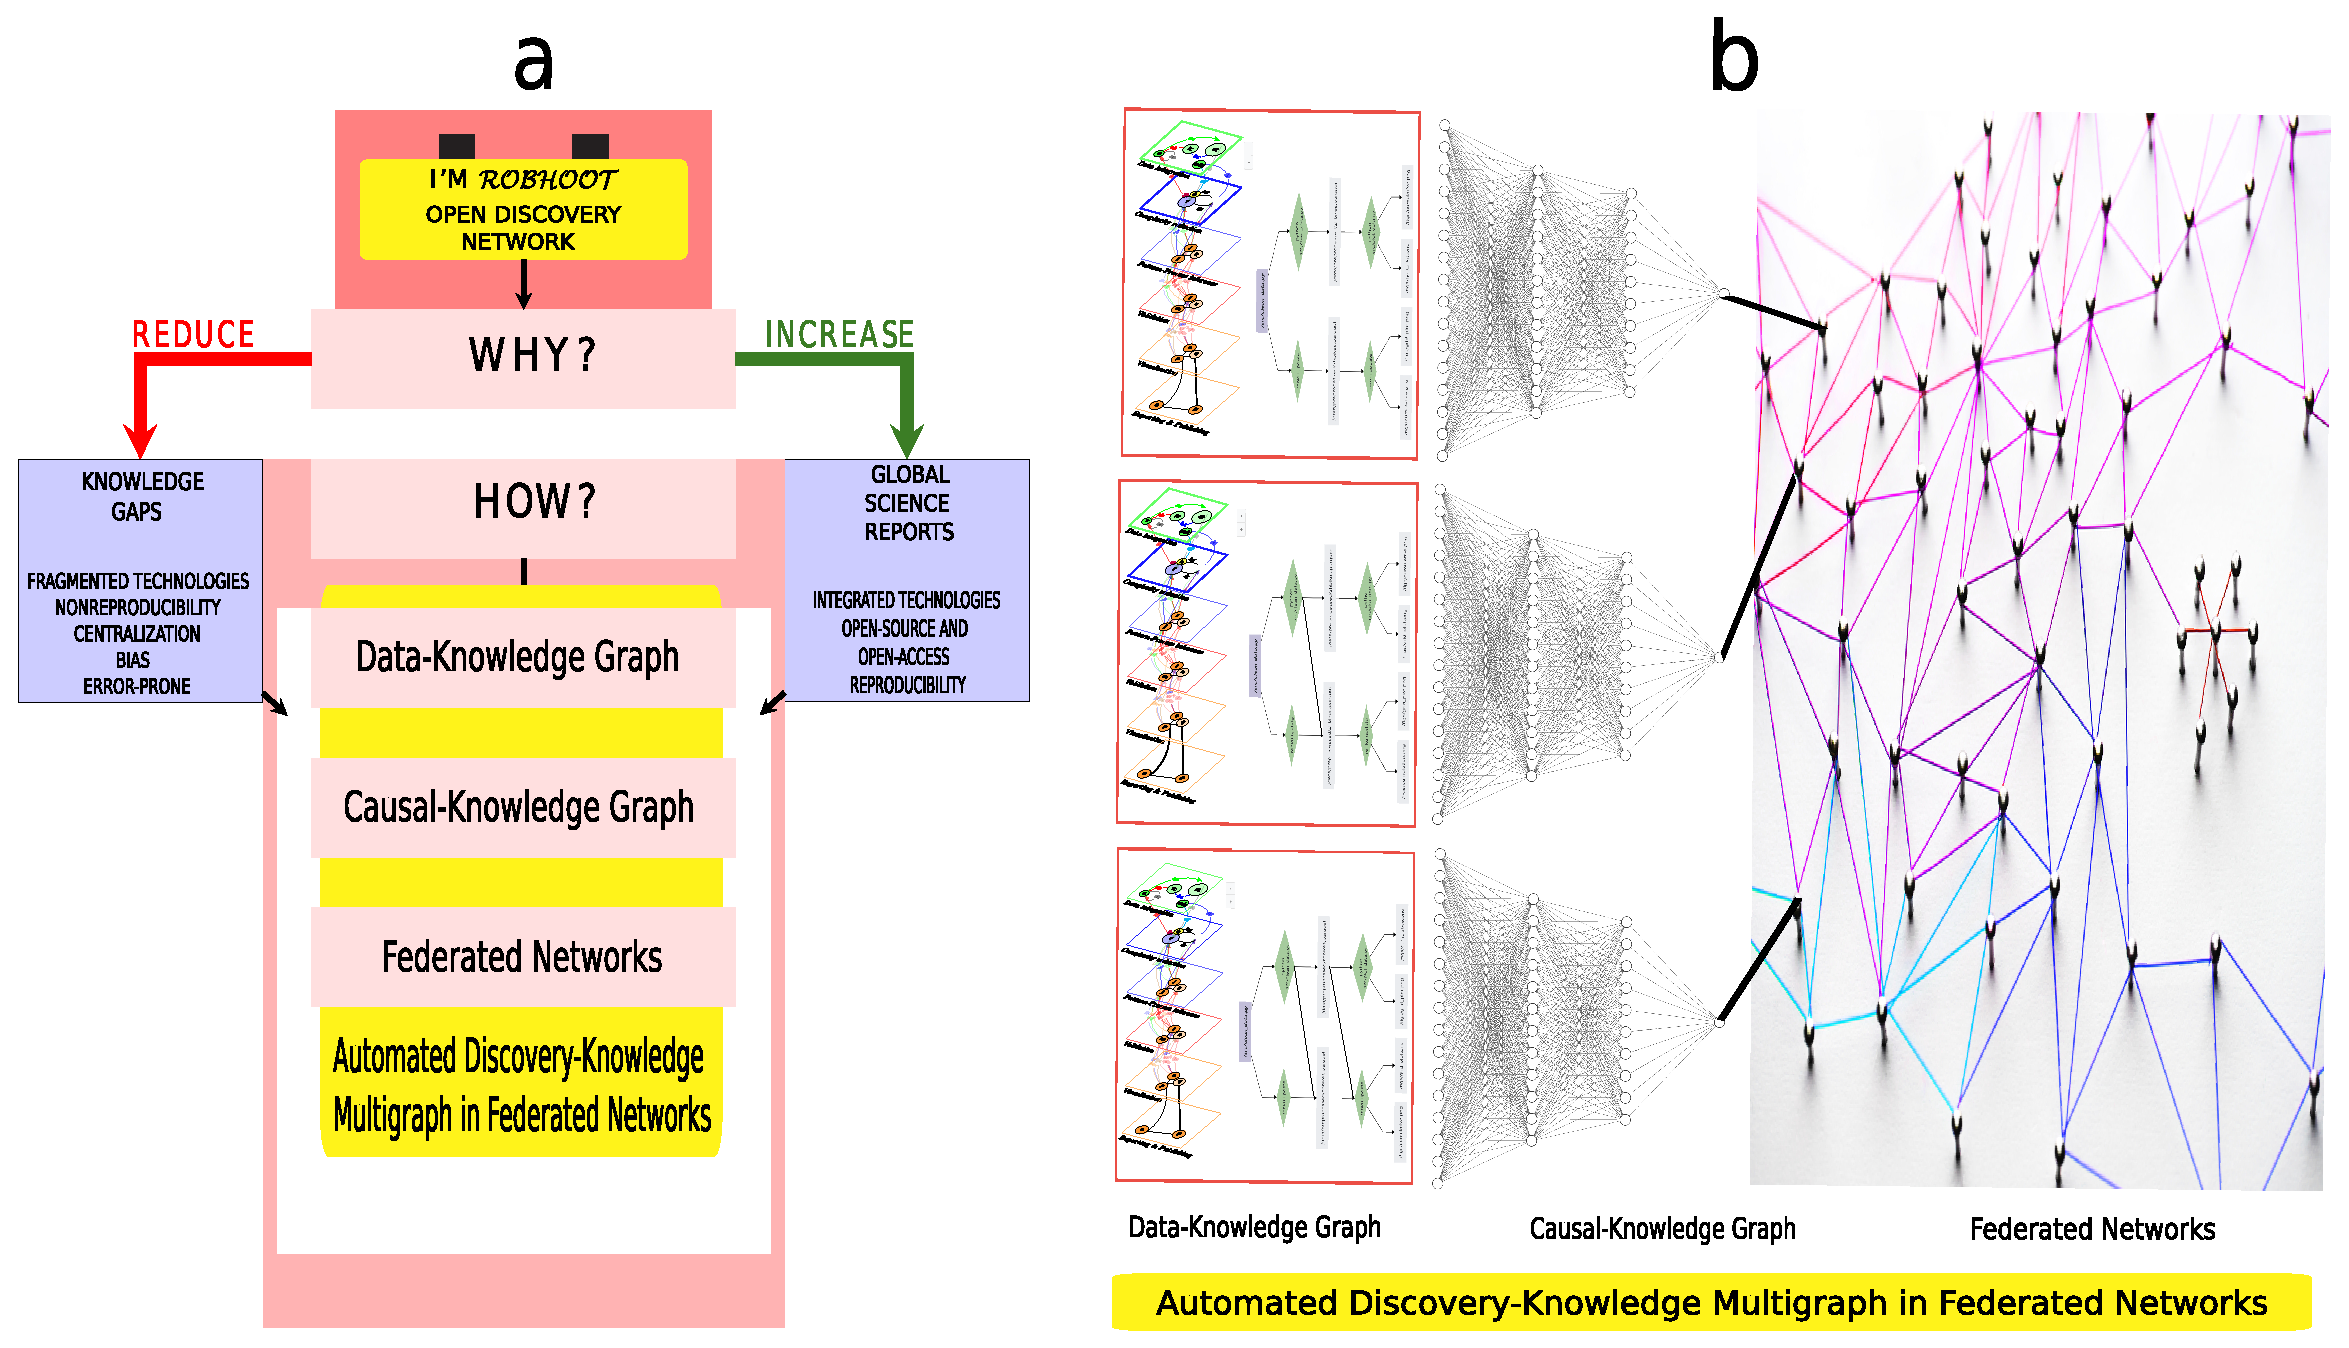
\includegraphics[width=1\textwidth]{Figures/AutomatedDiscovery.pdf}
    \caption*{\small {\bf Figure 1: Discovery in Evolutionary
        Biology-Inspired Federated Networks}. $\mathcal{ROBHOOT}$
      fussion data and causal knowledge graphs, the ``Discovery
      Knowledge Graphs'', into biology-inspired federated networks for
      a sustainable knowledge-inspired society: {\bf a)}
      $\mathcal{ROBHOOT}$ targets global knowledge gaps (red path) and
      open-access reproducible discovery reports (green path). It
      introduces three core science-enabled tehcnologies: {\bf a,b)}
      Data knowledge graphs to merge heterogeneous data-sources from
      semantic evolutionary algorithms for data discovery. {\bf a,b)}
      Causal Knowledge Graphs to fussion data knowledge to
      interpretable patterns using ``Evolutionary AI automation''
      algorithms, and {\bf a,b)} Discovery in biology-inspired
      federated networks for ``Cooperative Forecasting''. Taken
      together, the three core science-enabled technologies form the
      {\bf discovery knowledge graphs in evolutionary biology-inspired
        federated networks}, a compact technology integrating data and
      causal knowledge graphs into federated networks to generate
      cooperative forecasting in the face of biodiversity and
      sustainability challenges.}}
\end{figure}

%--------------------Summary------------------------Out of the draft -----------------------------
\begin{comment}
 The Robhoot project is trying to introduce new concepts to allow
  scientist and the public to interact in a decentralized open-access
  knowledge network to gain informed decisions when solving complex
  social, environmental and technological problems. Current
  technologies for scientific inquiry are highly fragmented and thus
  only increase robustness, reproducibility and the interactions with
  the public marginally (refs). The goal of Robhoot is to propose a
  new hybrid-technology concept combining deep learning, automation
  and distributed ledger technology with the advances of neural
  biological networks to lay the foundation for a novel open-science
  ecosystem aiming to couple predictive and knowledge power in
  contemporary societies. Robhoot is not set out to deliver a finished
  deep knowledge ledger network in the science ecosystem but provide a
  science-enabled technology in establishing a prototype
  proof-of-principle for an open public-science ecosystem.
 
\begin{table}
 %\rowcolor{pink}
\begin{tabular}{ p{6cm} | p{3cm} | p{3cm}}
  \hline \hline
  \textbf{Features} & \textbf{Science Ecosystem} &\textbf{{\bf $\mathcal{ROBHOOT}$}}\\  \hline
  Decentralization & No & Yes \\ \hline
  Full automation & No & Yes \\ \hline
  Open-access & Mostly No & Yes \\ \hline
  Immutability & No & Yes \\ \hline
  Robustness & Mostly No & Yes \\ \hline
  Reproducibility & Mostly No & Yes \\ \hline        
  Owner-Controlled assets & No & Yes \\ \hline       
  \bottomrule
\end{tabular}
\caption{{\bf $\mathcal{ROBHOOT}$} is designed to resolve desirable
  properties of science: Open-access, immutability, robustness,
  reproducibility, and owner-controlled assets. These features will be
  added during the different stages of development of the project
  (section ``Design Goals'').}
\end{table}
\end{comment}
%----------------------------------------------------------------------------------------------

   
\begin{table*}[ht]
 %\rowcolor{pink}
\begin{tabular}{ p{6cm} | p{11cm}}
  \hline \hline
  \textbf{Word} &\textbf{Meaning}\\  \hline
  Data knowledge graph & Graph obtained from merging heterogeneous data-sources \\ \hline
  Causal knowledge graph & Explainable/interpretable pattern inference from heterogeneous data-sources \\ \hline
  % Evidence-based knowledge gap & Solid scientific knowledge facing
  % constraints to be transfered to benefit society\\ \hline
  % Research-based knowledge gap & Differential access to the research
  % knowledge limiting information transfer to the society \\ \hline
  Discovery knowledge graph & Fussion of data and causal knowledge graphs for novel mechanistic inference of heterogeneous data\\ \hline
  %Reproducible knowledge graph & High-resolution tracking of the research cycle to make it fully open and transparent\\ \hline
  Automation & Algorithms targeting minimal human-driven interference\\ \hline
  Knowledge inspired society & Open-access discovery to facilitate informed decisions in global sustainability challenges \\ \hline
  Neutral-knowledge generation & Reproducible reports making transparent the many sources of bias in the discovery process\\ \hline
  \bottomrule
\end{tabular}
\caption{{\bf Glossary of terms.}}
\end{table*}

\subsection{Science-to-technology breakthrough that addresses this vision}

Interconnected global societies are constantly facing new challenges
that need to be rapidly addressed. In this regard, technologies
integrating data-driven causal inference into intelligent networks
providing rapid discovery when solving complex governance, social,
environmental and technological problems are lacking. Depite rapid
advances of research platforms for data analytics in the last decade
\citep{Melniketal:2010,Steinruecken,Modulos,Guimera2020,GoogleAI,IrisAI,easeml,datarobot,aito},
the integration of science-enabled technologies currently lack
discovery knowledge-inspired approaches impacting knowledge-inspired
societies to help responding to the rapidly changing global
sustainability challenges (Figures 1 and 2, and Table 1). Discovery
technologies facilitating understanding of complex systems still
present many challenges ({\bf +++}). This is particularly relevant in
global sustainability landscapes, where data heterogeneity like
different sampling efforts, many sampling methods, data fragmentation,
and lack of transparency limit our understanding of empirical patterns
to predict new emerging situations more accurately (Figure 2).

Our understanding of evolved information processing systems driven by
multidimensional factors and highly heterogeneous groups is currently
quite limited. \textcolor{red}{Discuss the relevant state-of-the-art
  and the extent of the advance the project would provide beyond this
  state-of-the-art. How will $\mathcal{ROBHOOT}$ go beyond
  state-of-the-art? $\mathcal{ROBHOOT}$ introduces biology-inspired
  explainable knowledge graphs into federated networks accounting for
  heterogeneity and multidimensionality to make discovery a rapidly
  evolving feature in digital ecosytems (Figure 2). How will
  $\mathcal{ROBHOOT}$ explicitly deal with diversification and
  dimensionality when accounting for highly heterogeneous evolving
  groups and interactions? (refs about federated networks, bacterial
  consortia, federated bacteria..., artificial life, problem solving
  artificial societies, and large-scale meta-learning in the federated
  setting \citep{Dilley2016}). Describe the science-to-technology
  breakthrough, targeted by the project that would represent the first
  proof of concept of the envisioned technology.} Patterns from
knowledge-graphs are emerging at a fast pace in specific frontiers
{\bf +++}, but remains isolated from the discovery process especially
in the context of cooperative discovery in federated networks {\bf
  +++}. $\mathcal{ROBHOOT}$ goes beyond the state-of-the-art of
knowledge-graphs by fussioning data and causal knowledge graphs, the
discovery knowledge graphs, and scalating these into evolving
biology-inspired federated networks to move knowledge-inspired
societies towards reaching global sustainability goals when large
number heterogeneous groups share resources driven by multiple
factors.}

{\bf $\mathcal{ROBHOOT}$ v.1.0} deploys a data discovery technology to
generate data knowledge graphs for an understanding of interpretable
patterns accounting for heterogeneous data-sources. Data-architecture
alone is not sufficent to outline predictive scenarios in complex
sustainability problems. Therefore, data analytics complementing
data-architecture discovery is desirable to interpret scenarios in
natural and digital ecosystems. In this regard, there are also many
gaps in connecting global data-architecture into rapid automated
causal knowledge graphs, the discovery knowledge graphs, to facilitate
discovery. {\bf $\mathcal{ROBHOOT}$ v.2.0} integrates automated and
explainable evolutionary biology-inspired methods to decipher causal
knowledge graphs from open-ended modeling scenarios. Still, rapidly
drawing scenarios from a few labs limit the parameter phase space from
where the discovery process is generated. Therefore, the scalability
of fully reproducible discovery strongly depend on cooperation and
learning in large scale biology-inspired federated networks. {\bf
  $\mathcal{ROBHOOT}$ v.3.0} brings discovery knowledge graphs to
federated networks by connecting heterogeneous-neural inspired
networks to learning to obtain cooperative forecasting from
heterogeneous collections of data-sources (section 3.3).

\subsection{Interdisciplinarity and non-incrementality of the research
  proposed}

\textcolor{red}{Respond more directly! --- Explain why the proposed
  research is non-incremental --- Describe the research disciplines
  necessary for achieving the targeted breakthrough of the project and
  the added value from the interdisciplinarity:: Still in a
  descriptive phase here:: Now it is a disconnected set of ideas} {\bf
  $\mathcal{ROBHOOT}$} is a science-enabled multi-feature technology
for interpretable data-driven discovery in federated networks (Figures
1 to 3 and Tables 1 to 3). It contains three milestones each
characterized by a mixture of research disciplines. {\bf
  $\mathcal{ROBHOOT}$ v.1.0} is composed by computer scientists,
evolutionary biologists and developers targeting novel evolutionary
inspired algorithms for API data discovery. This module is
complemented with scientists from complex networks taking care of
quantitative methods in the data knowledge graphs to decipher the
existing gaps in data discovery and data-architecture technologies
(section 3.1). {\bf $\mathcal{ROBHOOT}$ v.2.0} team is compossed by
data-scientists trained in deep learning networks and automation
algorithms, theoreticians and biologists with expertise in modeling
mechanistic and Bayesian networks and biology-inspired neural
networks, respectively. The combination of data-scientists,
theoreticians and biologists generates a diverse team targeting
synthesis between automated and explainable evolutionary
biology-inspired approaches to decipher causal knowledge graphs from
heterogeneous data-sources (section 3.2). {\bf $\mathcal{ROBHOOT}$
  v.3.0} combines computer scientists and developers targeting sharing
and evolutionary biology-inspired models of federated networks, with
social scientist, and scientists specialized in ecology and
evolutionary biology (section 3.3). The complementarity of the teams
in modules one to three strengthen the collaboration for making
$\mathcal{ROBHOOT}$ a science-enable functional technology in a
rapidly evolving digital ecosystem \citep{Soto-Valero2019}.

\textcolor{red}{$\mathcal{ROBHOOT}$ aims to bring global transparency
  in knowledge generation by acting as an assistant or as an automated
  and reproducible discovery generator to facilitate sustainability
  goals in ecosystems. The multi-feature, science-enabled technology
  target a reduction in global knowledge gaps while transparently
  accounting for centralization \citep{Inhaber1977,Gunther2018}⁠⁠, bias⁠⁠
  \citep{Ioannidis2005}, error-prone \citep{Fang2011}, and
  non-reproducibility \citep{Hardwicke2018} (Figures 1 and 2 and Table
  1). These features are mostly due to the rapidly evolving digital
  ecosystem. For example, it is increasing continuously its computing
  capacity, new methods integrating automated and explainable AI are
  rapidly advancing, and their interconnection to open-source
  technologies is also rapidly occurring in the digital ecosystem {\bf
    +++}. Yet, targeting automated data and causal knowledge graphs
  into federated networks still require taking risky steps: combining
  heterogeneous data-sources and evolutionary biology-inspired neural
  modeling approaches to fill out the existing gaps in the explainable
  methods arena ato bring them to causal inference of learning with
  heterogeneous agents sharing resources in complex ecosystems.}

  \begin{comment}
  Yet, technologies with the capacity to compactly accounting for neutral,
  borderless, immutable, and open-access information in hybrid,
  trusted-untrusted peer-to-peer interactions, accounting for the
  multilayer nature of science and engineering are currently not in
  place. We have already advanced in the integration of the different
  modules, from the automated identification, retrieval and data
  integration to inference and process-based discovery. We have
  implemented a prototype for the ongoing covid-19 pandemic (section
  3.3). Each module includes state-of-the-art developments in computer
  science, complex systems, and theoretical evolutionary ecology. The
  proof- of-concept is not fully automated yet and still requires
  human intervention in module integration and the development of a
  testnet stage. Nonetheless, we are currently exploring innovative
  solutions especially in the modules of automated data discovery,
  causal-knowledge graphs, reporting, and visualization.  Producing
  such a technology will require integrating expertise from disparate
  disciplines like multilayer networks, deep learning, automation
  algorithmics, and distributed technologies. The integration of these
  disciplines will require to go beyond domain boundaries.
\end{comment}

%Renku, Fabric and gitchain.

\subsection{High risk, plausibility and flexibility of the research approach}


\begin{itemize}
\item \textcolor{red}{Explain how the research approach relates to the
    project objectives and how it is suitable to deal with the
    considerable science-and-technology uncertainties and appropriate
    for choosing alternative directions and options. (The risks and
    mitigation plan should be spelled out under the Implementation
    section).}
\end{itemize}

\begin{comment}
  Knowledge-inspired societies and governance will demand full
  research cycle transparency, reproducibility and interpretability to
  inform complex social, environmental and technological problems. The
  need of transparency, reproducibility and interpretability brings
  many technical and functional challenges to our research proposal
  because obtaining robust knowledge from integrating many parts each
  containing its own set of methods can generate divergent, fragile
  and contradictory outcomes. {\bf $\mathcal{ROBHOOT}$} will have a
  modular and flexible structure following four main versions each
  divided in four work packages and milestones.
\end{comment}

\begin{comment}
  We will develop a flexible research method focusing more in the
  algorithmic robustness of the deep ledger knowledge network than in
  the development of robust automated knowledge generation. Our
  motivation will be to provide a first proof of concept of how the
  technology works: we will sample the KGs using different deep
  learning algorithms to estimate the uncertainty of the ruled-based
  inference obtained by fitting predictions to simulated data (Goal
  G1). Accounting for the uncertainties of each of the research stages
  when sampling the KGs comes from the many distinct paths within and
  across the layers in the research cycle (Figure 1). We will test a
  variety of consensus algorithms to explore the degree of security,
  decentralization and scalability of the ledger knowledge network
  using the generated population of KGs (Goal G2). Despite our focus
  will be bias towards the side of the algorithmic robustness of the
  deep ledger knowledge network, we will develop a domain-specific
  case study, our Robhoot Open Network, to test the robustness of the
  rule-based inference obtained by fitting each of the generated KG to
  the empirical patterns (Goal G3). The high risk associated to
  robustly automate the full research cycle for producing immutable
  open knowledge is buffered to a great extend because the existing
  ecosystem of tested and reliable open-source tools: We will combine
  our own algorithms (i.e., data integration and deep learning
  algorithms for sampling and automating the KGs) with open-source
  tools like Renku, Fabric and gitchain. This open-ecosystem will
  allow us to have a flexible launching of a testnet to collect data
  to explore the security-scalability-decentralization patterns and
  the robustness of the generated KGs in the deep ledger knowledge
  network (Goal G4.)
\end{comment}



%============IMPACT====================================================
\section{Impact}
\label{cha:impact}


\subsection{Expected impact} 
\label{sec:expected-impact}
\instructions{
  \textit{Please be specific, and provide only information that applies to the proposal and its objectives. Wherever possible, use quantified indicators and targets.}\\
  
\begin{itemize}
\item {\bf Scientific and technological contribution (to the foundation of a new future technology)}:\\
  $\mathcal{ROBHOOT}$ target novel approaches towards sustainable
  ecosystems. One of the tasks in WP3 will focus on the discovery of
  novel evolutionary-inspired algorithms to provide results for
  sustainability fisheries. These solutions will ultimately be
  developed from merging WP3 with the rest of WP's. For example, it is
  known that sustainable ecosystems strongly depend on many data
  sources collected by different groups using different
  technologies. Accounting for such heterogeneity combining fishery,
  stakeholders, and technology data, the data knowledge graph, with
  the technological and environmental changes and processes underlying
  the empirical patterns, the causal knowledge graphs, will provide a
  solid set of results for understanding sustainability in
  human-disturbed ecosystems. Altogether, this project will lay the
  foundation for future sustainability studies. Discovery of novel
  evolutionary-inspired algorithms for biodiversity maintenance have
  been hardly been investigated in this context so far. Therefore,
  several predictors related to biodiversity, technological and social
  times series analysis will be tested and further developed to enable
  robust prediction of sustainability. The discovery of new solutions
  not observed in the empirical data, but containing the highest
  degree of biodiversity and sustainability, will be the basis for
  estimation of the severity of overfishing and sampling bias when
  many groups enter in commercial conflict of interest. Such a
  targeted sustainability proxies would be of great interest not only
  for the biodiversity maintenance but also from an economic and
  social point of view, as it would save costs for future
  generations. Sustainability challenges are related to the
  development of future sustainable societies, which according to
  (Organization) ....
  
\item {\bf Potential for future social or economic impact or market creation}:\\
  \textcolor{red}{Describe the importance of the technological outcome
    with regards to its transformational impact on science, technology
    and/or society:} Collapse of ecosystems can lead to serious long
  term economic and ecological disfunctionalities. However, there are
  no established markers for the characterization of sustainability
  measures in complex ecosystems. Our approach accounts for
  heterogeneous sources of data, the mechanisms underlying
  technological, environmental and social changes required to make
  ecosystems sustainable and novel rules that could impact positively
  the maintenance of biodiversity by developing cooperative
  forecasting strategies among the many groups involved. Such a risk
  assessment would not only be of great interest to the groups
  exploiting the resources, but also from an economic and ecological
  point of view, as having less bias in the field data provides more
  accurate measures from the observed time series for planning fish
  stocks. Finally, $\mathcal{ROBHOOT}$ contributes towards
  knowledge-inspired societies in need of radically tackling new
  societal and global environmental challenges: it provides
  reproducible and transparent methods for making sustainability goals
  achievable and reproducible across many sectors and economies.

  In the medium-term this technology may also have interesting
  applications in public and private XXX industry. For example, access
  to discovery with cooperative forecasting might suggest new paths
  and solutions that are key to generate rapid and robust scenarios
  when facing complex problems including global sustainability
  challenges (i.e., global health, ecosystems degradation,
  biodiversity loss, etc). First, evolutionary AI automation decipher
  open-ended search interpretation of complex systems for private and
  public industry facing highly heterogeneous data sources. Second,
  cooperative forecasting challenges existing fragmented responses to
  emergent global sustainability problems by compactly offering
  reproducible forecasting emerging from many-to-many human and
  machine cooperative discovery, and third, open-access explainable
  and automated information generation account for global
  data-arquitecture allowing individuals and companies to address
  scenarios of future strategies in highly fluctuating local and
  global market conditions.

\item {\bf Impact on transparency and reproducibility}:\\
  Decision making and governance at local, regional and global scales
  require access to transparent and reproducible information
  containing data-architcture, interpretable factors generating the
  empirical patterns and novel algorithms suggesting future
  directions. \textcolor{red}{Make clear here the Choirat and Guimera
    group about reproducibility and automation in each of the
    Milestones, respectively. Explicitly mention about Legal and
    financial transparency -- Reproducibility in Social Governance --
    Impact to emerging and sustainability challenges :: Novel service
    for NGO, society and thinktank transparent and reproducible public
    policies: Advisory boards. Check the SDG -- This consortium brings
    together excellent partners from the fields of computer science,
    neurobiology, complex system, biology and evolutionary ecology and
    including one SME, who all exhibit a long-standing experience
    interdisciplinary research across the boundaries of the individual
    disciplines (Figure 3). The subsection on related projects shows
    that this is a novel constellation in Europe (and possibly
    worldwide. This consortium is also at the leading edge
    of...}... $\mathcal{ROBHOOT}$ target global automated,
  transparent, reproducible, and explainable discovery with a large
  impact on knowledge-inspired societies in need to access robust and
  reproducible reports to take informed decisions when facing...{\bf
    Keep elaborating}
  
\item {\bf Ecosystem health impact}: {\bf How will $\mathcal{ROBHOOT}$
    impact Ecosystem health?} The main value proposition of this
  proposal is the novel discovery of solutions for ecosystem
  sustainability challenges. Being able to provide novel discovery
  paths to ... By 2030 organization X suggest technologies around
  sustainability discovery will form Y percent of global
  economies...{\bf Keep elaborating}

\item {\bf Building leading research and innovation capacity across Europe}:\\
  \textcolor{red}{Building leading research and innovation capacity
    across Europe by involvement of key actors that can make a
    difference in the future, for example excellent young researchers,
    ambitious high-tech SMEs or first-time participants to FET under
    Horizon 2020} This consortium brings together excellent partners
  from the fields of computer science, machine learning, deep learning
  networks, neurobiology, complex systems, experimental biology,
  biology and evolutionary ecology and in particular evolutionary
  biology-inspired federated networks both from a theoretical and an
  experimental point of view, Physics, theory and applications of
  complex systems in social networks and one highly innovative
  science-based communication focusing on sustainability
  solutions. The use of advanced evolutionary biology-inspired and
  complex networks-based analyses to characterize and predict novel
  discovery in systems formed by heterogeneous and evolving groups and
  interactions combined with the implementation of intelligent
  learning discovery in federated networks and the development of a
  reproducible and automated protocol user friendly interface go much
  beyond the current state-of-the-art in science-based discovery
  technologies. All consortium partners exhibit a long-standing
  experience in interdisciplinary research across the boundaries of
  the individual disciplines (Show this in Figure 3). The subsection
  on related projects shows that this consortium is at the leading
  edge of innovation and interdisciplinarity. A significant value
  proposition of the project is to increase the research on
  large-scale sustainable federated networks where many agents share
  resources embedded in complex ecosystems. This will produce valuable
  information and data about how federated networks work under broad
  set of socio-ecological scenarios, similar to natural ecosystems
  consoritiums where many paths produce coexistence of heterogneous
  poulations and high biodiversity. It is important to consider that
  all ecosystems facing many human pressures are all across the world
  and discovery technologies facilitating the solutions in large-scale
  federated networks could inspire new developments improving our
  understanding of sustainability at global scale. For in-home, we
  also expect an explosion of discovery knowledge approaches and
  future publications, which will place Europe at the top of
  sustainability in federated networks.

  Moreover, in WPX, we propose the generation of a web-based
  sustainability discovery portal that will allow researchers, NGO,
  managers and the public to train students in the discovery process
  to manage over-exploited ecosystems, allowing to scale up the number
  of people participating in the sustainability process by an order of
  magnitude thus mobilising forward thinking researchers and excellent
  young researchers to work together and explore what may become a new
  technology paradigm in sustainability research. Members of the
  consortium already have experience in generating such types of
  training tools that are currently available online (check github
  repository RobhooX) in use in... This approach would provide an
  unprecedented capability for the access to a multitude of people
  interested in sustainability tools that will result in generating a
  consensus and a valuable source of information for science-enabled
  technologies in ecosystem sustainability and management.
\end{itemize}
 
  
\subsection{Measures to maximize impact} 
\label{sec:maximize-impact}

\textcolor{red}{This section still collection of what to follow ++
  random ideas}

%mention here the plan for reproducibility and automation
\subsubsection{Dissemination and exploitation of results}

\label{sec:dissemination-exploitation}
\instructions{
\begin{itemize}
\item \textcolor{red}{Provide a plan for disseminating and exploiting the project
  results. The plan, which should be proportionate to the scale of the
  project, should contain measures to be implemented both during and
  after the project.}
\item \textcolor{red}{Explain how the proposed measures will help to achieve the
  expected impact of the project.}
\item \textcolor{red}{Where relevant, include information on how the
    participants will manage the research data generated and/or
    collected during the project, in particular addressing the
    following issues:For further guidance on research data management,
    please refer to the H2020 Online Manual on the Participant
    Portal.}
\item \textcolor{red}{What types of data will the project generate/collect?}
\item \textcolor{red}{What standards will be used?}
\item \textcolor{red}{How will this data be exploited and/or
    shared/made accessible for verification and re-use? If data cannot
    be made available, explain why.}
\item \textcolor{red}{How will this data be curated and preserved?
    {\bf Choirat}: Reproducibility: Encode the Data-Knowledge graph
    into a Reproducible-Knowledge Graph using Renku.}
\end{itemize}

\emph{You will need an appropriate consortium agreement to manage (amongst other things) the ownership and access to key knowledge (IPR, data etc.). Where relevant, these will allow you, collectively and individually, to pursue market opportunities arising from the project's results.} \\
\emph{The appropriate structure of the consortium to support exploitation is addressed in section 3.3.}\\
\begin{itemize}
\item \textcolor{red}{Outline the strategy for knowledge management and protection. Include measures to provide open access (free on-line access, such as the ``green'' or ``gold'' model) to peer-reviewed scientific publications which might result from the project. Open access must be granted to all scientific publications resulting from Horizon 2020 actions. Further guidance on open access is available in the H2020 Online Manual on the Participant Portal.}\\
\end{itemize} 
\emph{Open access publishing (also called 'gold' open access) means that an article is immediately provided in open access mode by the scientific publisher. The associated costs are usually shifted away from readers, and instead (for example) to the university or research institute to which the researcher is affiliated, or to the funding agency supporting the research.}\\
\emph{Self-archiving (also called 'green' open access) means that the
  published article or the final peer-reviewed manuscript is archived
  by the researcher - or a representative - in an online repository
  before, after or alongside its publication. Access to this article
  is often - but not necessarily - delayed (``embargo period''), as
  some scientific publishers may wish to recoup their investment by
  selling subscriptions and charging pay-per-download/view fees during
  an exclusivity period.}
\end{itemize}
}

\begin{itemize}
\item \textcolor{red}{Connect to the consortium part taking care of Reproducibility and Automation}
\item \textcolor{red}{Strategic dissemination and exploitation will help to
  explain the wider societal relevance and long-term economic impact
  of science, build support for future research and innovation
  funding, ensure uptake of results within the scientific community,
  open up potential business opportunities for novel products or
  services, and potentially contribute to better decision-making
  processes and serve as valuable input for public policies
  formulation.  Dissemination: General dissemination targets are
  scientists, decision-makers, business community and the public.
  General dissemination measures will focus on project results and
  stakeholder engagement (stakeholder consultation processes;
  workshops to raise awareness, etc.) through:
  \\
  G1. The project website will be set up within the first three months
  of the project.
  \\
  G2. Up to date information material, e.g. brochures, presentation
  slides, will be distributed at events to increase awareness about
  our project.
  \\
  G3. General other publication means will be used such as newspapers,
  YouTube, TV and radio, social networks (e.g., Facebook) as well as
  targeted mailing lists (e.g., AI-worldwide).
  \\
  G4. Scientific publications for the scientific community. We will
  target high-level journals with open access, like Science, Nature
  Communication, etc.
  \\
  G5. The consortium will visit conferences in the related scientific
  fields in order to interactively present and discuss our results
  with others. Among other activities, the consortium will organize
  special sessions at several conferences.  Additionally, some
  targeted, specific dissemination actions will be considered: S1. We
  need to address mainly multipliers and developers in the ¿??¿? AI
  community?¿?  who engage in data processing. This will be achieved
  by a “traveling salesman” approach using personal visits and
  invitations to demonstrate our system.??  S2. Target groups need to
  be specified and addressed.  These are mainly: X departments in
  relevant companies in the sectors????  S3. At the end of the project
  we will organize a workshop specifically on X?? approaches for
  disseminating our results in ??? for assessing future exploitation
  potential, inviting partners from academia as well as industry.
  \\
  1. G4 will launch a testnet to help disseminate the main results of
  the deep ledger knowledge network. The launch will have invited
  NGO’s and GO across disciplines and social, economical and
  technological sectors.
  \\
  2. The Robhoot Open network will be launched as a Biodiversity
  research network to integrate the existing public databases and
  crowdsource data collections into the automated KGs and ledger
  network to facilitate NGOs, GO and other organizations transparency
  and governance in Biodiversity management.
  \\
  3. The project aims to publish its main findings in top open
  scientific journals to communicate the global impact of a deep
  ledger knowledge network for transparency and governance across
  social and economical sectors.}


\subsubsection{Communication activities}
\label{sec:communication}
\instructions{
\begin{itemize}
\item \textcolor{red}{Describe the proposed communication measures for
    promoting the project and its findings during the period of the
    grant. Measures should be proportionate to the scale of the
    project, with clear objectives.  They should be tailored to the
    needs of various audiences, including groups beyond the project's
    own community. Where relevant, include measures for
    public/societal engagement on issues related to the project.}

\item \textcolor{red}{Data management and accessibility to community: Other
  than being constrained by possible IPRs, Robhoot strictly adheres to
  the Open Access Policy of the Commission and all publishable
  (non-protected) results will follow the green or gold OA
  policy. Software as well as hardware protocols will be made openly
  available through standard computer science repositories such as
  GitHub. Data (measured data), as such, will not be acquired by
  Robhoot. Open-source framework for delay analysis Standardized
  inputs and software will be made public through an online platform
  with the aim of converting it in The Reference Point for any future
  research in delay propagation modeling. Open access to publications
  will be granted under the terms and conditions laid down in the
  Grant Agreement, in accordance with the Rules for participation and
  dissemination in Horizon 2020. The beneficiaries will deposit an
  electronic copy of the published version or the final manuscript
  accepted for publication of a scientific publication relating to
  foreground in an institutional or subject-based repository at the
  moment of publication, e.g., via the OpenAIRE portal
  (www.OpenAIRE.eu). In addition, beneficiaries will make their best
  efforts to ensure that this electronic copy becomes freely and
  electronically available to anyone through this repository (i.e.,
  that it becomes “open access”): immediately, if the scientific
  publication is published “open access”, i.e., if an electronic
  version is also available free of charge via the publisher, or
  within 6 months of publication.}}
\end{itemize}

\section{Implementation}

A technology deciphering data and causal knowledge graphs to tackle
global problems related to sustainability challenges is highly
informative by itself, but a diverse group of scientists across Europe
have decided to connect discovery and sustainability broadly. We want
to advance cooperative discovery in the global digital ecosystem. To
this end, the $\mathcal{ROBHOOT}$ consortium aims at integrating data
and causal knowledge graphs, the discovery knowledge graphs, into
evolving federated networks to achieve cooperative forecasting for
global sustainability challenges. $\mathcal{ROBHOOT}$'s goals are
developed in three main milestones and ten deliverables (Tables
3.1a-c).

\begin{figure}[h!]
  %\centering
   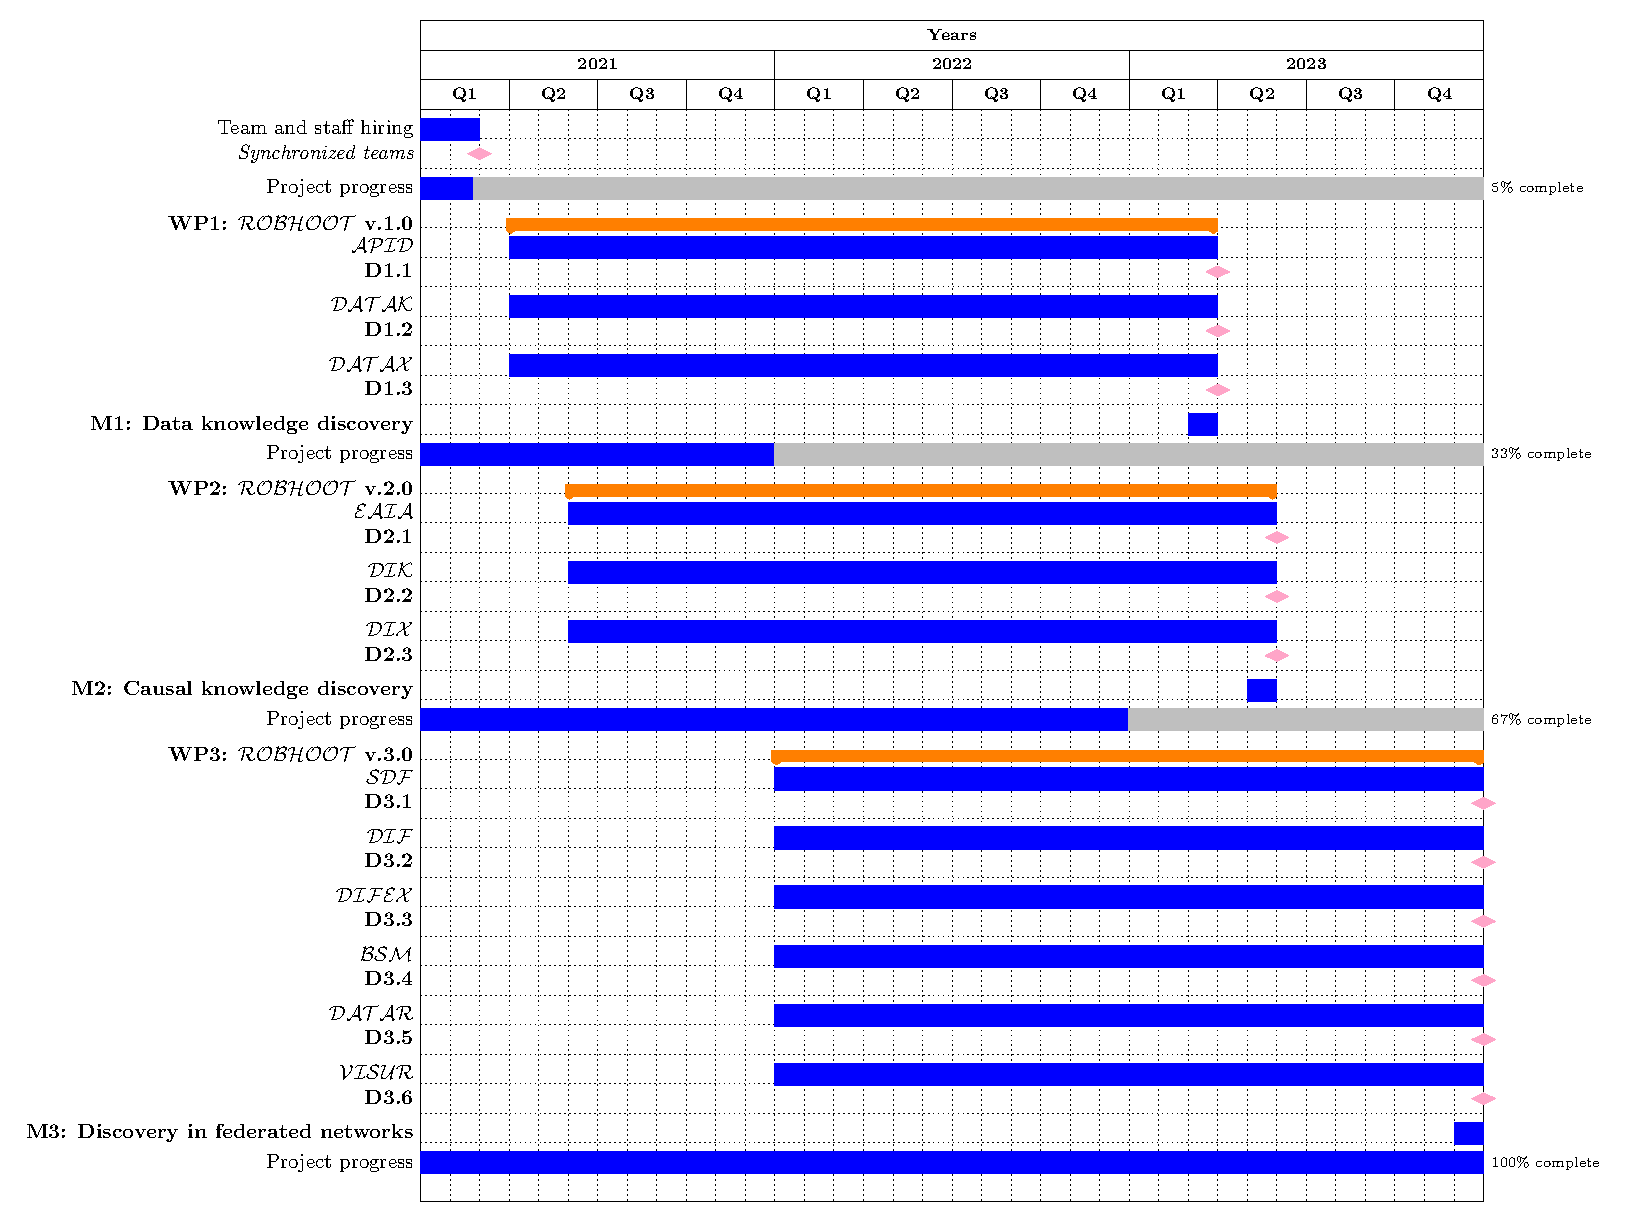
\includegraphics[width=1\textwidth]{Figures/GanttChart.pdf}
   \caption*{{\small {\bf Table 3.1a: $\mathcal{ROBHOOT}$ Gantt
         Chart}: Work package one, {\bf WP1}, introduces Milestone
       {\bf $\mathcal{ROBHOOT}$ v.1.0} and deliverables {\bf D1.1} to
       {\bf D1.3} to generate the data knowledge graph for the
       Exploration of the Seas Network (Figure 2). Work package two,
       {\bf WP2}, introduces {\bf $\mathcal{ROBHOOT}$ v.2.0} and
       deliverables {\bf D2.1} to {\bf D2.4} to fussion data and
       causal knowlede graphs into interpretable patterns, the
       discovery-knowledge graphs for the Exploration of the Seas
       Network. Work package three, {\bf WP3}, introduces {\bf
         $\mathcal{ROBHOOT}$ v.3.0} and deliverables {\bf D3.1} to
       {\bf D3.3} to discover knowledge graphs from biology-inspired
       evolving federated networks.}}
\end{figure}

  
\subsection{Research methodology and work plan , work packages,
  deliverables}

\subsubsection{{\bf WP1: $\mathcal{ROBHOOT}$ v.1.0}: \\ Data Knowledge
  Graphs}


\textcolor{blue}{API discovery technologies to build robust and
  scalable automated data-driven discovery is an existing need
  \citep{Fan2012,Staar2018}. Technologies around building database are
  particularly relevant to generate explainable (or interpretable)
  Artificial Intelligence technologies for global emergency or
  sustainability landscapes where new questions and scenarios are
  constantly emerging and new data is constantly being added to a
  large pool of servers \citep{Futia2020}. Building database from a
  large pool of heterogeneous data, however, comprises a series of
  privacy requirements, formats, dimensions, biases and spatiotemporal
  resolution that constraint data integration and discovery
  \citep{Openstreetmap,Bluecloud,HOT,Elixir}. Fortunately, standard
  protocols to automate API discovery, semantic knowledge extraction,
  and ETFs algorithms are rapidly advancing
  \citep{Fan2012,APISGURU,OpenKnowledgeFoundation}, and overall
  different types of semantic technologies are rapidly emerging in the
  context of integrating many datasets into data knowledge graphs
  \citep{KGcovid19}. Yet, technologies focusing on evolutionary
  semantic knowledge extraction algorithms to build data knowledge
  graphs from many heterogeneous API and data-sources that can be
  rapidly integrated into interpretable technologies are not currently
  in place \citep{Futia2020} (\textcolor{red}{make clear how
    evolutionary biology-inspired semantic knowledge extraction
    algorithms might work}. $\mathcal{ROBHOOT}$ v.1.0 explores
  science-enabled technologies around heterogeneous API data-discovery
  along three main deliverables (Table 3.1a-b, {\bf D.1.1} to {\bf
    D.1.3} and Figure 3). $\mathcal{ROBHOOT}$ v.1.0 generates a data
  knowledge graph from heterogeneous data-sources for the exploration
  of the Seas network. $\mathcal{ROBHOOT}$ v.1.0 explores evolutionary
  biology-inspired rules using sematic algorithms to discover API and
  interactions that can be added to the exploration of the Seas
  database. (Keep elaborating here) Focus will be in complementing the
  existing exploration of the Seas database containing 9 million
  entries, 1612 species, around 20 countries and 11 sampling methods
  (Figure 2) expandint it with Fishery data, species interactions and
  social and stakeholders groups with different interests within each
  of the countries involved in the international exploration of the
  Seas.}


 %Word package description
\begin{table}[h!]
\begin{center}
  \begin{tabular}{|m{3cm} || m{12cm} || m{1cm}|}
    \hline\hline\hline
    \rowcolor{lightpink!30}
    {\bf Work package} & & {\bf Lead Beneficiary} \\
    \hline
    \rowcolor{piggypink!20}
    {\bf Title} & {\bf $\mathcal{ROBHOOT}$ v.1.0} &  \\
    \hline
    \rowcolor{piggypink!20}
    {\bf Participants} & {\bf Fortuna, Egu\'iluz, Choirat} & \\
    \hline
    \rowcolor{piggypink!20}
    {\bf Person Month per participant} & & \\
    \hline
    \rowcolor{piggypink!20}
    {\bf Start month} & {\bf 3} & \\
    \hline
    \rowcolor{piggypink!20}
    {\bf End month} & {\bf 27} & \\
    \hline
    \rowcolor{piggypink!20}
    {\bf Objectives} & Data Knowledge Graph & \\
    \hline
    \rowcolor{piggypink!20}
    {\bf Description} & Extraction diverse data-sources to infer data knowledge graphs & \\
    \hline
    \rowcolor{piggypink!20}
    {\bf Deliverables} & {\bf D1.1 ($\mathcal{APID}$}): Heterogeneous API and data discovery
                         {\bf D1.2 ($\mathcal{DATAK}$}): Heterogeneous data knowledge graph
                         {\bf D.1.3 ($\mathcal{DATAX}$}): Data knowledge graph for the exploration of the Seas network & \\
    \hline\hline\hline
    \rowcolor{piggypink!20}
    {\bf Title} & {\bf $\mathcal{ROBHOOT}$ v.2.0} &  \\
    \hline
    \rowcolor{piggypink!20}
    {\bf Participants} & {\bf Baity, Guimer\`a, Meli\'an, Vicente} & \\
    \hline
    \rowcolor{piggypink!20}
    {\bf Person Month per participant} & & \\
    \hline
    \rowcolor{piggypink!20}
    {\bf Start month} & {\bf 5} & \\
    \hline
    \rowcolor{piggypink!20}
    {\bf End month} & {\bf 29} & \\
    \hline
    \rowcolor{piggypink!20}
    {\bf Objectives} & Causal Knowledge Graph & \\
    \hline
    \rowcolor{piggypink!20}
    {\bf Description} & Interpretable knowledge extraction from data knowledge graphs & \\
    \hline
    \rowcolor{piggypink!20}
    {\bf Deliverables} & {\bf D2.1 ($\mathcal{EAIA}$}): Automated biology-inspired AI algorithms        
                         {\bf D2.2 ($\mathcal{DIK}$}): Discovery evolutionary biology-inspired knowledge graphs
                         {\bf D2.3 ($\mathcal{BSM}$}): Bayesian causal-knowledge graphs                
                         {\bf D2.4 ($\mathcal{DIX}$}): Discovery knowledge graphs for the exploration of the Seas network  & \\
    \hline \hline\hline
    \rowcolor{piggypink!20}
    {\bf Title} & {\bf $\mathcal{ROBHOOT}$ v.3.0} &  \\
    \hline
    \rowcolor{piggypink!20}
    {\bf Participants} & {\bf von Waldow, Maass} & \\
    \hline
    \rowcolor{piggypink!20}
    {\bf Person Month per participant} & & \\
    \hline
    \rowcolor{piggypink!20}
    {\bf Start month} & {\bf 18} & \\
    \hline
    \rowcolor{piggypink!20}
    {\bf End month} & {\bf 42} & \\
    \hline
    \rowcolor{piggypink!20}
    {\bf Objectives} & Biology-inspired Evolving Federated Network & \\
    \hline
    \rowcolor{piggypink!20}
    {\bf Description} & Automated discovery knowledge graphs in federated networks & \\
    \hline
    \rowcolor{piggypink!20}
    {\bf Deliverables} & {\bf D3.1 ($\mathcal{SDF}$}): Sharing discovery knowledge graphs in federated networks
                         {\bf D3.2 ($\mathcal{DIF}$}): Discovery in biology-inspired federated networks 
                         {\bf D2.3 ($\mathcal{DIFX}$}): Discovery in biology-inspired exploration of the Seas federated networks  & \\
    \hline\hline\hline
  \end{tabular}
\end{center}
\caption*{{{\bf Table 3.1b Work package description}: Work package,
    Title, Participants, Person Months per participant, Start and End
    month, Objectives, Description and deliverables of each Work
    Package.}}
\end{table}

\subsubsection{{\bf WP2: $\mathcal{ROBHOOT}$ v.2.0}: \\
  Causal Knowledge Graphs}

AI is rapidly advancing as an automated and explainable technology
making more transparent predictions for complex and multidimensional
datasets
(\citep{OHare2015,Gil2019,Cranmer2019,Guimera2020,Real2020,Futia2020},+++). This
is particularly relevant in Earth, Ecosystem and Sustainability
science, where merging automation to interpretable and mechanistic
understanding of data might increase human ability to make stronger
inferences about future sustainability challenges and solutions
\citep{Reichstein}. $\mathcal{ROBHOOT}$ v.2.0 explores the causal
mechanisms underlying heterogeneous and multidimensional landscapes by
integrating open-ended automated evolutionary biology-inspired
solutions, AI methods and Bayesian space models along four main
deliverables (Table 3.1a-c, {\bf D.2.1} to {\bf D.2.4} and Figure
2). $\mathcal{ROBHOOT}$ v.2.0 deploys milestone ``Evolutionary AI
automation'' (Figure 3.1a-c) to search evolutionary algorithms to
decipher the meaning of the interactions and the nodes in evolving
networks, the causal knowledge graph (Figure
2). \textcolor{blue}{$\mathcal{ROBHOOT}$ v.2.0 introduces the
  ``Evolutionary AI automation'' algorithm for the exploration of the
  Seas case study as follows: the use of different Gears between
  Ireland and Spain makes fish species catchability different. This
  produces a strong bias in the distribution maps (compare Megrim
  vs. Haddock map, Figure 2) while countries' preference is biased
  towards their own fishery interest. Groups can be represented with
  evolving environmental and technological traits. This can be
  formally described as a distribution-fishery
  cooperation-competition matrix,  $\mathcal{C}^2$, as follows: \vspace{0.1 in}\\
\begin{center}
  $\mathcal{C}^2$ = \bordermatrix{~ &
    $\mathcal{F}^{i}_{\mathcal{A}_{g},\mathcal{B}_{g}}(c)$ &
    $\mathcal{F}^{i}_{\mathcal{A}_{g},\mathcal{B}_{g}}(nc)$ \cr
    $\mathcal{D}^{i}_{\mathcal{A}_{g},\mathcal{B}_{g}}(c)$ &
    $c(\varphi)$ & $c(\Phi), nc(\gamma_{A_{g}},\gamma_{B_{g}})$ \cr
    $\mathcal{D}^{i}_{\mathcal{A}_{g},\mathcal{B}_{g}}(nc)$ &
    $nc(\Phi_{A_{g}},\Phi_{B_{g}}), c(\gamma)$ &
    $nc(\phi_{A_{g}},\phi_{B_{g}})$ \cr}, \vspace{0.2 in}
\end{center}
\\
where $\mathcal{D}$, $\mathcal{F}$, $i$, $\mathcal{A}_{g}$,
$\mathcal{B}_{g}$, c and nc, represent Distribution map and Fishery of
species $i$, group $g$ within country $\mathcal{A}$ and $\mathcal{B}$,
cooperation and non-cooperation, respectively. We will automate
evolving functions representing environmental and technological traits
with different degrees of complexity in the $\mathcal{C}^2$ matrix: If
the two groups within the countries cooperate, $c(\varphi)$, then the
environmental and technological rate change, $\varphi$, is
syncrhonized between groups to evolve towards decreasing Gear bias and
make distribution maps and the fishery sustainable. On the other side,
if the two groups decide not to cooperate,
$nc(\phi_{A_{g}},\phi_{B_{g}})$, then there is environmental and
technological rate change, $\phi_{A_{g}}$ and $\phi_{B_{g}}$ with each
group following changes of their own gears, the GOV for the Ireland
group and the Baka Gear for Spain group, independently of the other
and as a function of their Fishery interest. There is no interest in
decreasing bias in species distribution maps making fishery non
sustainable in this case. In the last two scenarios groups enter in
cooperation for the distribution map of species $i$, but not in the
Fishery ($c(\Phi), nc(\gamma_{A_{g}},\gamma_{B_{g}})$), or they do
cooperate in the Fishery for species $i$ but not for the distribution
map of species $i$ ($nc(\Phi_{A_{g}},\Phi_{B_{g}}), c(\gamma)$). The
situation for cooperation in the distribution maps follows agreements
between the two groups to technological changes in the Gear but still
preserving their GOV and the Baka Gears for
Fisheries. $\mathcal{ROBHOOT}$ v.2.0 search discovery knowledge graphs
for the exploration of the Seas (Figure 2) containing 9 million
entries, 1612 species, 15 countries and 11 sampling methods
contrasting predictions from evolutionary biology-inspired algorithms
in the framework of automated Bayesian machines ensuring the search,
the evaluation of models, trading-off complexity, fitting to the data
and quantify resource usage \citep{Guimera2020,Steinruecken}. Causal
knowledge graphs connect automated and explainable AI throughout
prediction and knowledge power (Figure 2).}

\begin{comment}
  I have trouble understanding the details of the KG in fig. 2: are
  there only edges between neightboring columns of nodes (if not,
  perhaps you want to draw this differently, arranging the clusters of
  nodes around the perimeter of a circle, like in the plot of
  connections between brain areas (see att.).

  Can you also give an example what knowledge a concrete edge in this
  KG could encode?  You write that is supposed to represent a causal
  KG. How does this affect the content of the edges?

  It would be very helpful if you could also give for this fish domain
  some concrete examples for the KGs that are considered in WP1, 2, 3,
  and the new methods and insights that these WPs are intended to
  produce for this fish example? This would help me to get an idea of
  the methods that would be needed for this.
\end{comment}


   \vspace{0.15 in}
   \begin{figure}[h!]
     \centering
     \hspace{-0.5 in}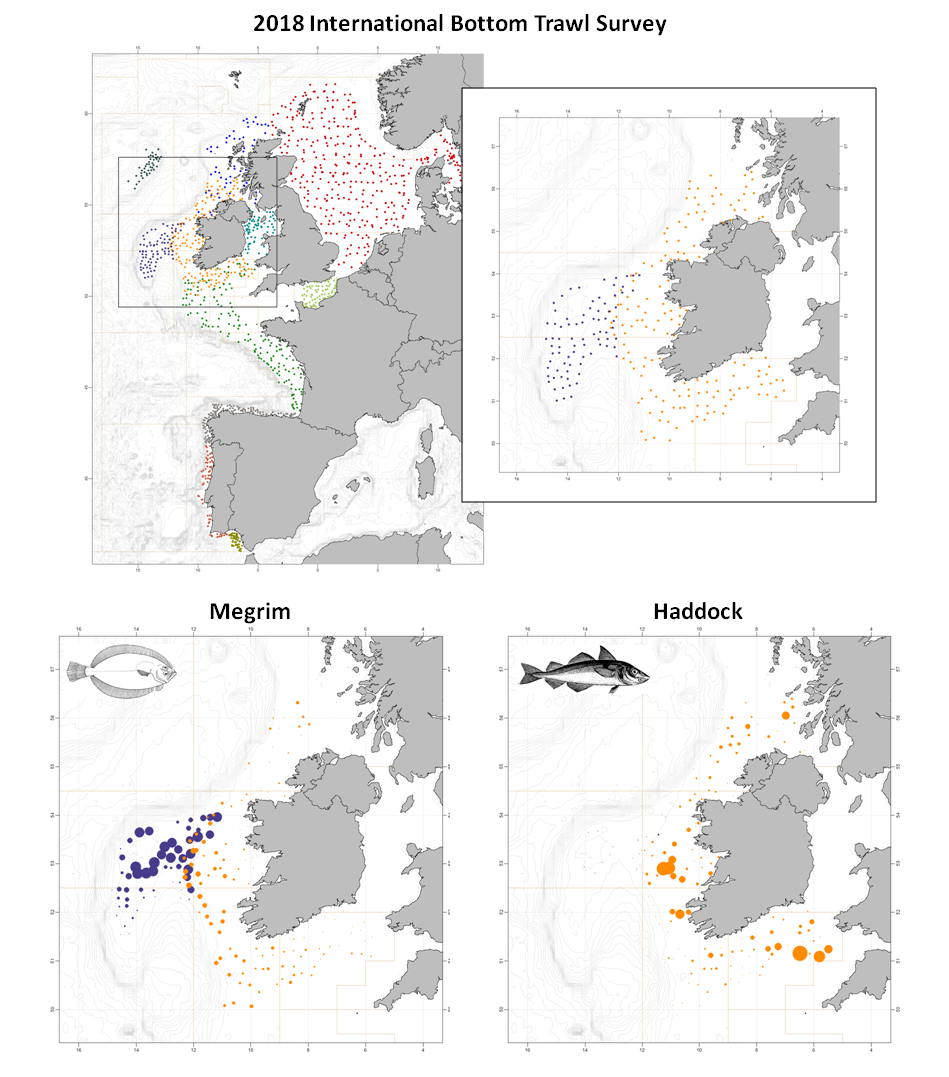
\includegraphics[width=14cm,height=10cm]{Figures/Figura.png}%Figure3integrated.pdf}
     \\
      \hspace{-0.5 in}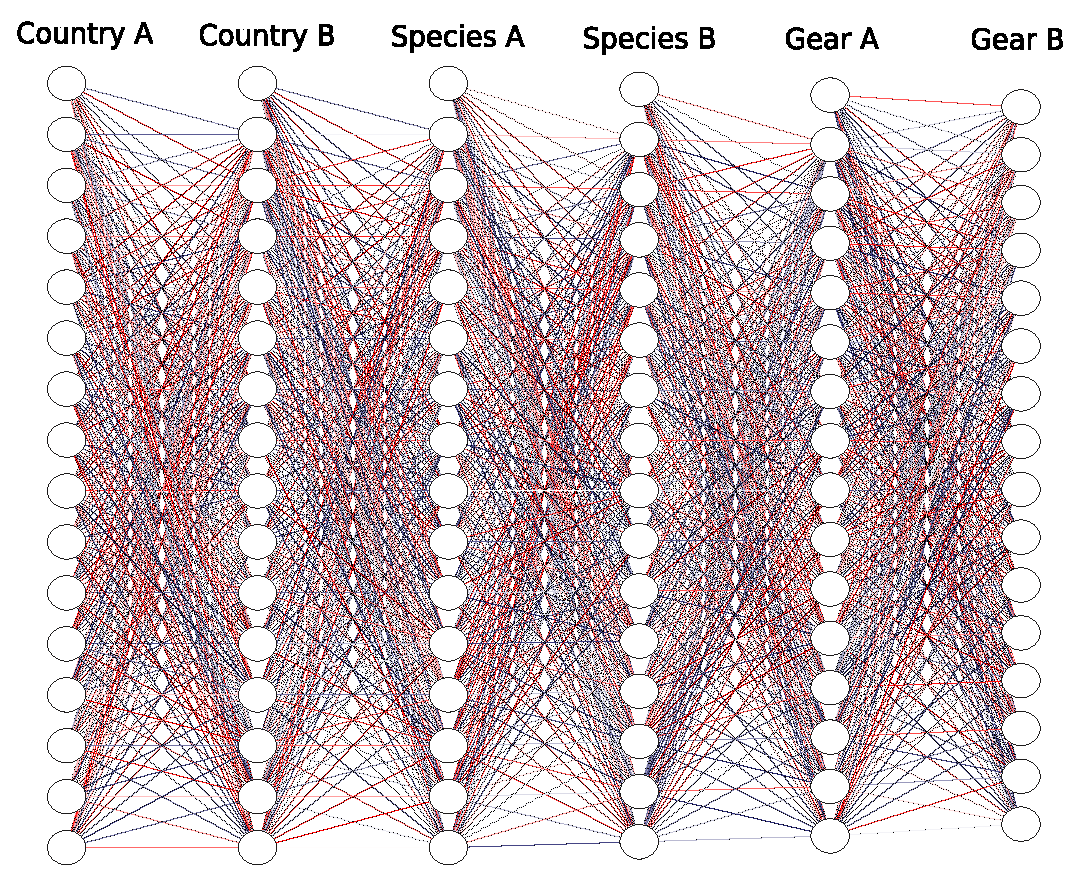
\includegraphics[width=12cm,height=6cm]{Figures/CKG.pdf}%Figure3integrated.pdf}
     \caption*{\small {\bf Figure 2: Causal Knowledge Graphs}.  {\bf
         Top}) The Irish Ground Fish Survey (IE-IGFS, Orange) and the
       Spanish Survey on the Porcupine Bank (SP-PORC, Blue) were part
       of the 2018 International Bottom Trawl Survey, coordinated by
       the International Council for the Exploration of the Sea
       \citep{ices}. Ireland and Spain use different Gears: The GOV
       gear has a larger vertical opening (Ireland, 3-4 m) respect to
       the Baka used on the Porcupine Bank (Spain, 2-3 m). This makes
       catchability different for fish species, such as Megrim
       ($Lepidorhombus$ $whiffiagonis$, {\bf Center left}) and Haddock
       ($Melanogrammus$ $aeglefinus$, {\bf Center right}), in which
       both countries have very different commercial
       interests. Haddock is a species of the cod family, highly
       prized in northern Europe, while Megrim is a species of
       flatfish, consumed largely in Spain and France. Spain catches
       Megrim better than Haddock and viceversa for Ireland. This
       generates a strong bias in the distribution maps (compare
       Megrim vs. Haddock map, Center). {\bf Bottom left}
       Causal-Knowledge Graph representing the 2-countries, 2-species
       and 2 gears example. The whole data set for 2018 contains 11
       countries, 461 fish especies (approx. 200k individuals
       sampled), and 5 gears. {\bf Bottom right}. Predictive-knowledge
       power map. x-axis represents ``Data-based inference'' (i.e.,
       gradient of non-interpretable ML methods from left (low) to
       right (high) predicting power). y-axis represents
       ``Process-based inference'' (i.e., gradient of process-based
       methods from bottom (low) to top (high) knowledge power). The
       gradient of predicting power map (top) shows a hot spot red
       area in the bottom right highlighting the region where AI best
       predict the empirical data. The gradient of knowledge power map
       (middle) shows a red hot spot in the top left highlighting the
       region where the best mechanistic understanding occur. The
       predicting-knowledge power map (bottom) shows the sum of the
       two previous maps highlighting a red hot spot where predicting
       and knowledge power occur.}}
\end{figure}


%Deliverable table  
\begin{table}[h!]
\begin{center}
  \begin{tabular}{|m{2cm} || m{1.25cm} || m{1.75cm} || m{1.55cm} || m{2.4cm} || m{1.7cm} || m{1.15cm} || m{1.7cm}|}
  \hline\hline
  \rowcolor{lightpink!30}
  {\bf $\mathcal{ROBHOOT}$ v.X.X} & {\bf Deliver. number} & {\bf Deliver. name} & {\bf WP} & {\bf Name Lead} & {\bf Type} & {\bf Disem.} & {\bf Delivery date} \\
  \hline\hline
  \rowcolor{piggypink!20}
  {\bf v.1.0} & {\bf D1.1} & $\mathcal{APID}$ & WP1 & {\bf Fortuna} & OT & PU & 27 \\
  \hline\hline
  \rowcolor{piggypink!20}
  {\bf v.1.0} & {\bf D1.2} & $\mathcal{DATAK}$ & WP1 & {\bf Egu\'iluz} & OT & PU  & 27 \\
  \hline\hline
  \rowcolor{piggypink!20}
  {\bf v.1.0} & {\bf D1.3} & $\mathcal{DATAX}$ & WP1 & {\bf Leads M1} & R,OT,DEC & PU  & 28 \\
    \hline\hline
 \rowcolor{piggypink!40}
  {\bf v.2.0} & {\bf D2.1} & $\mathcal{EAIA}$ & WP2 & {\bf Meli\'an} & OT & PU & 29 \\
  \hline\hline
  \rowcolor{piggypink!40}
  {\bf v.2.0} & {\bf D2.2} & $\mathcal{DIK}$ & WP2 & {\bf Baity/Vicente} & OT & PU  & 29 \\
  \hline\hline
   \rowcolor{piggypink!40}
  {\bf v.2.0} & {\bf D2.3} & $\mathcal{BSM}$ & WP2 & {\bf Guimer\`a} & OT & PU  & 29 \\
  \hline\hline
  \rowcolor{piggypink!40}
    {\bf v.2.0} & {\bf D2.4} & $\mathcal{DIX}$ & WP2 & {\bf Leads M2} & R,OT,DEC & PU & 30 \\
    \hline\hline
   \rowcolor{piggypink!60}
  {\bf v.3.0} & {\bf D3.1} & $\mathcal{SFN}$ & WP3 & {\bf von Waldow} & OT & PU & 42 \\
  \hline\hline
   \rowcolor{piggypink!80}
  {\bf v.3.0} & {\bf D3.2} & $\mathcal{DIF}$ & WP3 & {\bf Maass} & OT & PU & 42 \\
  \hline\hline
  \rowcolor{piggypink!80}
  {\bf v.3.0} & {\bf D3.3} & $\mathcal{DIFX}$ & WP3 & {\bf Leads M3} & R,OT,DEC & PU & 42 \\
\hline\hline
  \end{tabular}
\end{center}
\caption*{{{\bf Table 3.1c List of Deliverables}: {\bf
      $\mathcal{ROBHOOT}$} contains three main work packages: {\bf
      $\mathcal{ROBHOOT}$ v.1.0} span from Month 3 to 27. Deliverable
    {\bf D1.3 ($\mathcal{DATAX}$)} generates the data knowledge for
    the exploration of the Seas network. Milestone {\bf
      $\mathcal{ROBHOOT}$ v.2.0} span from Month 5 to 29. Deliverable
    {\bf D2.4 ($\mathcal{DIX}$)} generates the discovery knowledge
    graph for the exploration of the Seas network, and {\bf
      $\mathcal{ROBHOOT}$ v.3.0} span from Month 18 to 42, bringing
    the deliverable {\bf D3.3 (DIFX)}, discovery in biology-inspired
    exploration of the Seas network.}}
\end{table}

\subsubsection{{\bf WP3: $\mathcal{ROBHOOT}$ v.3.0}: \\
  Discovery Knowledge Graphs in Biology-Inspired Federated Networks}

Integrating data and causal knowledge graphs provide a mechanistic
understanding of how much cooperation vs. competition is occurring in
our exploration of the Seas case study. However, causal knowledge
graphs are not enough if they only represent isolated contributions
and can not ``learn to learn'' to find novel, emergent solutions in
biology-inspired networks composed by highly heterogeneous groups. In
this regard, federated objects can be seen as ``neural networks''
containing many types of heterogeneous nodes with varying degrees of
learning in the context of heterogeneity, connectivity and firing
probabilities \citep{Maass2014,Maass2015}. Technologies in digital
ecosystems around federated networks are scarce and mostly focus on
decentralization, scalability and security fronts
\citep{Golem2016,Dilley2016,Durov2017,Androulaki2018,OceanProtocolFoundation2018,BigchainDBGmbH2018}. In
the science ecosystem, only a few applications of open decentralized
technologies exist \citep{Gunther2018}. Yet, the discovery of novel
algorithms in biology-inspired federated networks for cooperative
forecasting of global sustainability problems when heterogeneous
groups learn and share from each other is currently not in place.

Recent studies have shown the importance of evolutionary search of
mathematical and symbolic operations as building blocks to discover ML
algorithms (\citep{Real2020,Guimera2020}). Evolutionary
biology-inspired search for algorithmic discovery can help to decipher
how interactions among heterogeneous groups evolve and learn to solve
complex sustainability problems. For example, evolutionary dynamics
can explore open-ended language of models with varying trait evolution
functions to discover biologically inspired solutions in
multidimensional systems (\citep{Real2020},+++). $\mathcal{ROBHOOT}$
v.3.0} deploys sharing discovery knowledge graphs, {\bf D3.1,
$\mathcal{SFN}$}, into biology-inspired federated networks accounting
for heterogeneous agents to discover novel biology-inspired solutions
for the exploration of the Seas federated network (Table 3.1a-c, {\bf
  D.3.1} to {\bf D.3.3}). \textcolor{red}{Can you also sketch concrete
  examples of what insight you aim at discovering in this case, and
  how automated discovery methods might provide new insight?}
Evolutionary algorithms might trigger novel algorithmic findings, the
discovery knowledge graphs, and \textcolor{blue}{$\mathcal{ROBHOOT}$
  v.3.0 introduces ``Cooperative Forecasting'' as evolutionary
  biology-inspired neural learning algorithms for discovery of new
  solutions in large federated networks (Figure
  3.1a-c). $\mathcal{ROBHOOT}$ v.3.0 search for how learning from
  interacting heterogeneous groups discover evolutionary algorithms
  and in our exploration of the Seas case study this can be
  represented as follows (In analogy from information processing and
  learning from heterogenous populations of neurons): Now the focus is
  on cooperative learning to discover new solutions. For example, how
  learning from the most distant strategies in the technological and
  environmental traits can make distribution catchability maps
  similar. Groups can now be represented not only as environmental and
  technological traits, but with evolving learning traits as a
  function of the distance between each pair of groups sharing
  resources. This can be formally
  described as a distribution-fishery cooperation learning matrix $\mathcal{C}^2$, as follows: \vspace{0.2 in}\\
\begin{center}
  $\mathcal{C}^2$ = \bordermatrix{~ & $\mathcal{F}^{i}_{\mathcal{A}_{g},\mathcal{B}_{g}}(c)$ & $\mathcal{F}^{i}_{\mathcal{A}_{g},\mathcal{B}_{g}}(nc)$ \cr
    $\mathcal{D}^{i}_{\mathcal{A}_{g},\mathcal{B}_{g}}(c)$ & $c(\varphi,\mathcal{L}_{d})$ & $c(\Phi,\mathcal{L}_{d}), nc(\gamma_{A_{g}},\gamma_{B_{g}})$ \cr
    $\mathcal{D}^{i}_{\mathcal{A}_{g},\mathcal{B}_{g}}(nc)$ & $nc(\Phi_{A_{g}},\Phi_{B_{g}}), c(\gamma,\mathcal{L}_{d})$ & $nc(\phi_{A_{g}},\phi_{B_{g}})$ \cr}, \vspace{0.2 in}
\end{center}
\\
where $\mathcal{D}$, $\mathcal{F}$, $i$, $\mathcal{A}_{g}$,
$\mathcal{B}_{g}$, c and nc, represent Distribution map and Fishery of
species $i$, group $g$ within country $\mathcal{A}$ and $\mathcal{B}$,
cooperation, and non-cooperation, respectively, as in
$\mathcal{ROBHOOT}$ v.2.0. In addition, we introduce learning
functions depending of the distance between two groups,
$\mathcal{L}_{d}$. We will search evolving learning functions that can
be coupled to environmental and technological traits with different
degrees of complexity in the $\mathcal{C}^2$ matrix: If the two groups
within the countries are sufficiently distant, then learning functions
play a role to cooperate, $c(\varphi, \mathcal{L}_{d})$, and the
environmental and technological rate change, $\varphi$, strongly
depend on learning between the interacting groups making distribution
maps and the fishery more sustainable.
(Write from here how the learning scenario can enter in the
non-cooperative strategies) On the other side, if the two groups
decide not to cooperate, $nc(\phi_{A_{g}},\phi_{B_{g}})$, then there
is environmental and technological rate change, $\phi_{A_{g}}$ and
$\phi_{B_{g}}$ with each group following changes of their own gears,
the GOV for the Ireland group and the Baka Gear for Spain group,
independently of the other and as a function of their Fishery
interest. There is no interest in decreasing bias in species
distribution maps making fishery non sustainable in this case. In the
last two scenarios groups enter in cooperation for the distribution
map of species $i$, but not in the Fishery
($c(\Phi), nc(\gamma_{A_{g}},\gamma_{B_{g}})$), or they do cooperate
in the Fishery for species $i$ but not for the distribution map of
species $i$ ($nc(\Phi_{A_{g}},\Phi_{B_{g}}), c(\gamma)$). The
situation for cooperation in the distribution maps follows agreements
between the two groups to technological changes in the Gear but still
preserving their GOV and the Baka Gears for
Fisheries. $\mathcal{ROBHOOT}$ v.2.0 search discovery knowledge graphs
for the exploration of the Seas (Figure 2) containing 9 million
entries, 1612 species, 15 countries and 11 sampling methods
contrasting predictions from evolutionary biology-inspired algorithms
in the framework of automated Bayesian machines ensuring the search,
the evaluation of models, trading-off complexity, fitting to the data
and quantify resource usage \citep{Guimera2020,Steinruecken}. }
 
Our understanding of the outcomes from evolved information processing
systems formed by highly heterogeneous groups, a kind of large-scale
meta-learning in the federated setting \citep{Dilley2016}, is
currently quite limited. Therefore, new science-enabled approaches
accounting for information processing with diversification of
heterogeneous and highly dimensional systems in federated networks are
required to develop science-enabled technologies where heterogeneous
agents with different interests find (non optimal)
solutions. $\mathcal{ROBHOOT}$ v.3.0 connects discovery knowledge
graphs to biology-inspired federated netwoks to study the properties
of cooperative forecasting and strong inference in the face of global
sustainability and biodiversity challenges (Figure 2 and Table
3.1.a-c).

\begin{comment}
\begin{table*}[ht]
 %\rowcolor{pink}
\begin{tabular}{ p{3.5cm} | p{14cm}}
  \hline \hline
  \textbf{Feature} &\textbf{$\mathcal{ROBHOOT}$}\\  \hline
  Long-term vision & Global open-access to a fully reproducible knowledge-generation inspired technology \\ \hline
  Breakthrough scientific and technological target & Collapsing evidence- and research-based knowledge gaps for a sustainable knowledge-inspired society\\ \hline
  Novelty & Science-based technology emerging from targeted algorithmic discovery at the interface of multilayer networks, knowledge graphs, deep-learning, and consensus mechanisms\\ \hline
  Foundational & Neutral-knowledge inspired technology for an emerging open science of science and science-society research disciplines \\ \hline
  High-risk & Adapted to explore new terrirories into the open-science-technology-society interface ecosystem \\ \hline
  Interdisciplinarity & Hybridizing expertise from distributed computing and deep learning to multilayer networks and the ecology and evolution of natural and digital ecosystems (Table 1) \\ \hline
  \bottomrule

\end{tabular}
\caption{{\bf $\mathcal{ROBHOOT}$} features along its developmental stages.}
\end{table*}
\end{comment} 



  \begin{comment}
    %\centering
  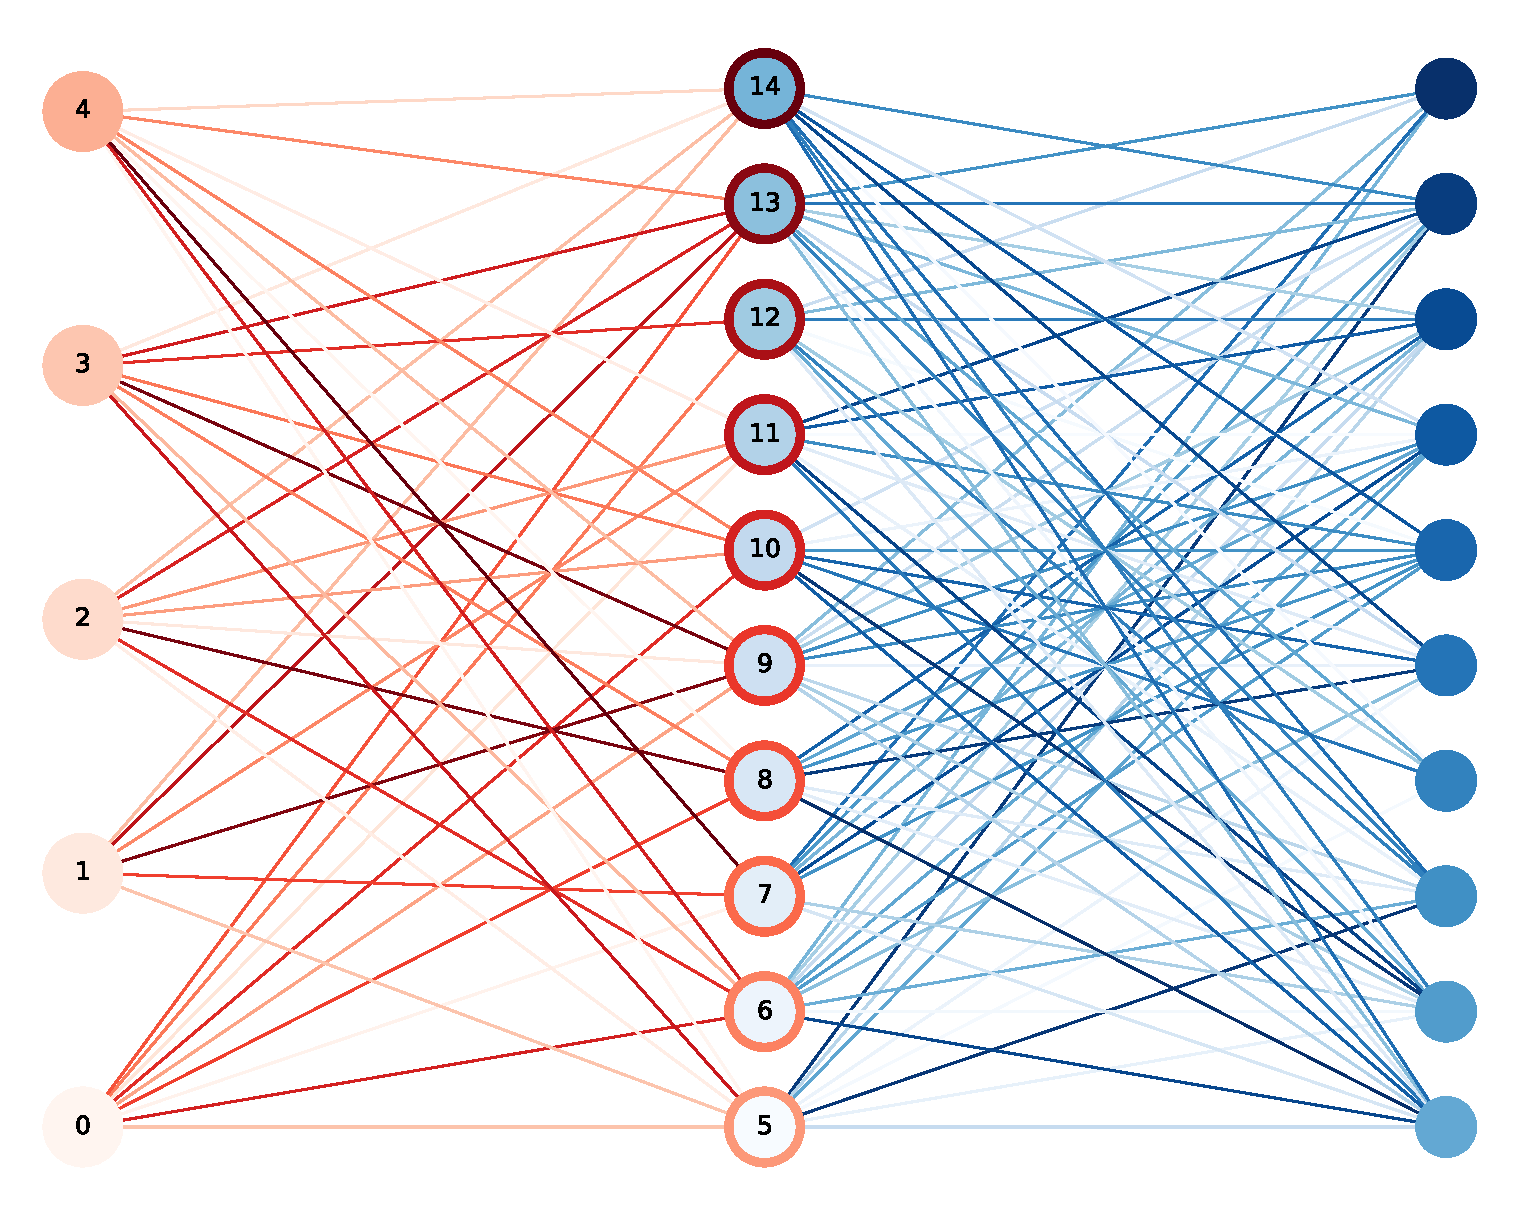
\includegraphics[width=0.45\textwidth]{Figures/FigureRobhoot.pdf}
 
  {\small {\bf Figure 3: Robhoot in Digital Ecosystems}: {\bf Left
      column}: {\bf $\mathcal{ROBHOOT}$ v.1.0} representing the
    research cycle as nodes from number 0 to 4: Data integration (0),
    Complexity Reduction (1), Inference (2), Validation (3), and
    Visualization(4)). {\bf Central column}: Nodes representing the
    research cycle in the left column are connected to open-source
    software in the digital ecosystem. Connections with node number 0
    in the left column can, for example, represent the ETLs
    open-source software interactions required to generate the {\bf
      Universal ETLs} module. The same meaning applies to the
    different nodes of the left column. {\bf Right column}: Each node
    represents a report meaning there is a reporting gradient
    generated by the connections to the open-source software from
    where each report is generated only using a subset of the research
    layers and open-source software.}
\end{comment}


\subsection{Management structure, milestones and procedures}

\begin{itemize}
  \item \textcolor{red}{Describe the organisational structure and the
      decision-making (including a list of milestones (table 3.2a))}
\item \textcolor{red}{Explain why the organisational structure and
  decision-making mechanisms are appropriate to the complexity and
  scale of the project.}
\item \textcolor{red}{Describe any critical risks, relating to project
    implementation, that the stated project's objectives may not be
    achieved. Detail any risk mitigation measures. Please provide a
    table with critical risks identified and mitigating actions (table
    3.2b) and relate these to the milestones.}
\end{itemize}

Advisory board covering the weakest parts of the proposal -- mention here

%Milestone table  
\begin{table}[h!]
\begin{center}
  \begin{tabular}{|m{1.75cm} || m{2.5cm} || m{2.5cm} || m{2.4cm} || m{6cm}|}
   \hline\hline
   \hline\hline
  \rowcolor{lightpink!30}
  {\bf Milestone number} & {\bf Milestone name} & {\bf Related work package(s)} & {\bf Due data (months)} & {\bf Verification} \\
   \hline\hline
   \rowcolor{piggypink!20}
  {\bf M1} & {\bf Data Knowledge Graph} & WP1 & 27 & OS-Software,Paper/Conf. &
  \hline\hline
  \rowcolor{piggypink!20}
  {\bf M2} & {\bf Evolutionary AI Automation}  & WP2 & 29 & OS-Software,Paper/Conf. &
  \hline\hline
  \rowcolor{piggypink!40}
  {\bf M3} & {\bf Discovery Knowledge Graph} & WP2-WP3 & 29 & OS-Software,Paper/Conf.,demo-website &
  \hline\hline
   \rowcolor{piggypink!60}
  {\bf M4} & {\bf Cooperative Forecasting} & WP3 & 42 & OS-Software,Paper/Conf.,main-website &
  \hline\hline
\hline\hline
  \end{tabular}
\end{center}
\caption*{{{\bf Table 3.2a: List of Milestones}: {\bf
      $\mathcal{ROBHOOT}$ v.1.0} span from Month 3 to 27 to generate
    the ``Data Knowledge Graph'' for the exploration of the Seas. {\bf
      $\mathcal{ROBHOOT}$ v.2.0} span from Month 5 to 29 producing the
    the Causal Knowledge Graph from the ``Evolutionary AI Automation''
    technology for the exploration of the Seas case study. {\bf
      $\mathcal{ROBHOOT}$ v.3.0} span from Month 18 to 42 to decipher
    ``Discovery Knowledge Graphs'' from ``Cooperative Forecasting'' in
    Biology-Inspired in Federated Networks.}}
\end{table}

  \subsection{Consortium as a whole}

  {\bf $\mathcal{ROBHOOT}$} is a science-enabled multi-feature
  technology. $\mathcal{ROBHOOT}$'s consortium is designed with a
  highly modular structure to gain milestone's functionality (Figure
  3, milestones from 1 to 3, blue, red, and pink,
  respectively). Connections among the modules reflect the emergence
  of interdisciplinarity technologies, the ``Discovery Knowledge
  Graph'', the ``Evolutionary AI Automation'' and the ``Cooperative
  Forecasting'' (Figure 3, green) \textcolor{red}{Is the
    interdisciplinarity in the breakthrough idea reflected in the
    expertise of the consortium? How do the members complement one
    another?}. {\bf $\mathcal{ROBHOOT}$ v.1.0}'s team is composed by
  Fortuna, Egu\'iluz and Choirat to bring data discovery process, to
  fully reproducible and heterogeneous knowledge graphs (section 3.1
  and Figure 3). Milestone one requires a mixture of researchers:
  computer-, data-scientists and developers and researchers working in
  complex networks from the quantitative and epistemological
  angles. Fortuna's, Egu\'iluz and Choirat's expertise complement each
  other's roles: Fortuna's team takes care of data knowledge graphs
  following evolutionary semantic algorithms for novel
  data-interactions and API discovery (i.e., {\bf $\mathcal{APID}$}
  and {\bf $\mathcal{DATAK}$, $\mathcal{DATAX}$}). Egu\'iluz's team
  focuses on network modularity, community detection and
  decentralization metrics for pattern detection in data knowledge
  graphs (i.e., {\bf $\mathcal{DATAK}$} and {\bf $\mathcal{DATAX}$},
  and Choirat's team encodes all the algorithms and procedures from
  Fortuna's and Egu\'iluz's teams into reproducible knowledge
  graphs. Milestone {\bf $\mathcal{ROBHOOT}$ v.1.0} generates a data
  knowledge graph for the exploration of the Seas (Figure 3, blue).

  {\bf $\mathcal{ROBHOOT}$ v.2.0}'s team composed by Guimer\`a, Baity,
  Vicente, and Meli\'an fussion Bayesian Machine Scientist to
  Evolutionary and AI Algorithms, forming the ``Evolutionary
  Automation'' approach (Figure 3, green). The ``Evolutionary
  Automation'' fussion data to causal knowledge graphs to make
  patterns interpretable (Figure 2). The team for this milestone add
  complementarity expertise to {\bf $\mathcal{ROBHOOT}$ v.1.0}'s team:
  Now the skills focus on data-scientists trained in deep learning
  networks and automation algorithms, theoreticians with expertise in
  Bayesian inference, and evolutionary biologists with expertise in
  evolutionary ecology theory and evolutionary-inspired networks
  (section 3.2 and Figure 3, red). Despite modules {\bf
    $\mathcal{ROBHOOT}$ v.1.0} and {\bf $\mathcal{ROBHOOT}$ v.2.0}
  focus on specific milestones and deliverables (Table 3.1a-c), they
  connect each other along data and causal knowledge graphs, the
  discovery knowledge graphs, and evolutionary automation to build a
  interdisciplinarity science-enabled technology that can be compactly
  converted into user-friendy open-software ({\bf Discovery Knowledge
    Graphs} and {\bf Evolutionary AI Automation}, green). Milestone
  {\bf $\mathcal{ROBHOOT}$ v.2.0} generates a discovery knowledge
  graph for the exploration of the Seas initially containing 9 million
  entries, 1612 species using around 11 sampling methods and more than
  15 countries (Figures 2 and 3, red). Thus, interdisciplinarity
  enters not only at the intra-module development stage, but also at
  the inter-module stage where discovery-knowledge graphs and
  evolutionary AI automation form the basis for a interdisciplinarity
  breakthrough reflected in the highly complementarity skills of the
  consortium (section 4.1). The first two modules in {\bf
    $\mathcal{ROBHOOT}$} contain researchers from Estonia, Spain,
  Switzerland and Sweden.
  
  The {\bf $\mathcal{ROBHOOT}$} consortium wants to advance the
  rapidly evolving digital ecosystem by making cooperative discovery a
  fundamental feature of it. For this purpose, a science-based
  automated and interpretable technology is not enough if each
  discovery knowledge graph stays isolated from one another. To
  contrast robustly interpretable scenarios in the face of global
  sustainability challenges, discovery knowledge graphs should learn
  to learn from heterogeneous data-sources in the contexxt of
  evolutionary biology-inspired federated networks. To achieve
  scalability for the discovery knowledge graphs, neural-inspired
  protocols in federated networks is the excellency feature of {\bf
    $\mathcal{ROBHOOT}$ v.3.0} (section 3.3). {\bf $\mathcal{ROBHOOT}$
    v.3.0}'s team composed by von Waldow and Maass, develops protocols
  for sharing discovery knowledge graphs along biology-inspired
  federated networks. The team forming {\bf $\mathcal{ROBHOOT}$ v.3.0}
  therefore requires quite a lot of contrasting skills. First,
  developers working in P2P and security protocols. Second, social
  scientists, computer scientists, and neurobiologists in
  collaboration to developers aiming to explore the role of
  heterogeneous groups of biology-inspired neurons accounting for
  heterogeneous data-sources in federated networks. Milestone {\bf
    $\mathcal{ROBHOOT}$ v.3.0} is a fundamental stepping-stone for
  developing ``Cooperative Forecasting'': it first guarantees
  discovery knowledge graphs are reproducible shareable objects. Yet,
  in the same way than evolutionary algorithms and the Bayesian
  machine scientist search automatically for open-ended space models
  to generate the plausible causal knowledge graphs, the discovery
  knowledge graphs produced in different nodes of a network need to
  automatically interact and learn from each other to find better
  forecasting scenarios at a global scale. {\bf $\mathcal{ROBHOOT}$
    v.3.0}'s implements heterogeneous groups of (cooperating and
  competing) neurons in federated networks for making cooperative
  forecasting a standard global property. Milestone {\bf
    $\mathcal{ROBHOOT}$ v.3.0} generates a discovery federated network
  for the exploration of the Seas to provide populations of scenarios
  satisfying biodiversity maintenance while guaranteeing commercial
  interest (Figure 3, pink). $\mathcal{ROBHOOT}$ v.3.0} contain
researchers from Switzerland and Austria.

\begin{figure}[h!]
  \floatbox[{\capbeside\thisfloatsetup{capbesideposition={right,top},capbesidewidth=4cm}}]{figure}[\FBwidth]
  {\caption*{Figure 3: $\mathcal{ROBHOOT}$ Consortium: {\bf
        $\mathcal{ROBHOOT}$ v.1.0} (blue) to {\bf $\mathcal{ROBHOOT}$
        v.3.0} (pink) with acronyms of each deliverable (Left column),
      tasks (Center), lead and partner names (Right columns). Links
      connect deliverables to tasks and leading/partners
      groups. $\mathcal{ROBHOOT}$ delivers three
      interdisciplinarity-driven science-enabled technologies: {\bf
        Discovery-Knowledge Graph} connecting {\bf $\mathcal{ROBHOOT}$
        v.1.0} and {\bf $\mathcal{ROBHOOT}$ v.2.0}. {\bf Evolutionary
        AI Automation} in {\bf $\mathcal{ROBHOOT}$ v.2.0}, and {\bf
        Cooperative Forecasting} connecting {\bf $\mathcal{ROBHOOT}$
        v.2.0} to {\bf v.3.0}}}
    %\label{fig:test}
  {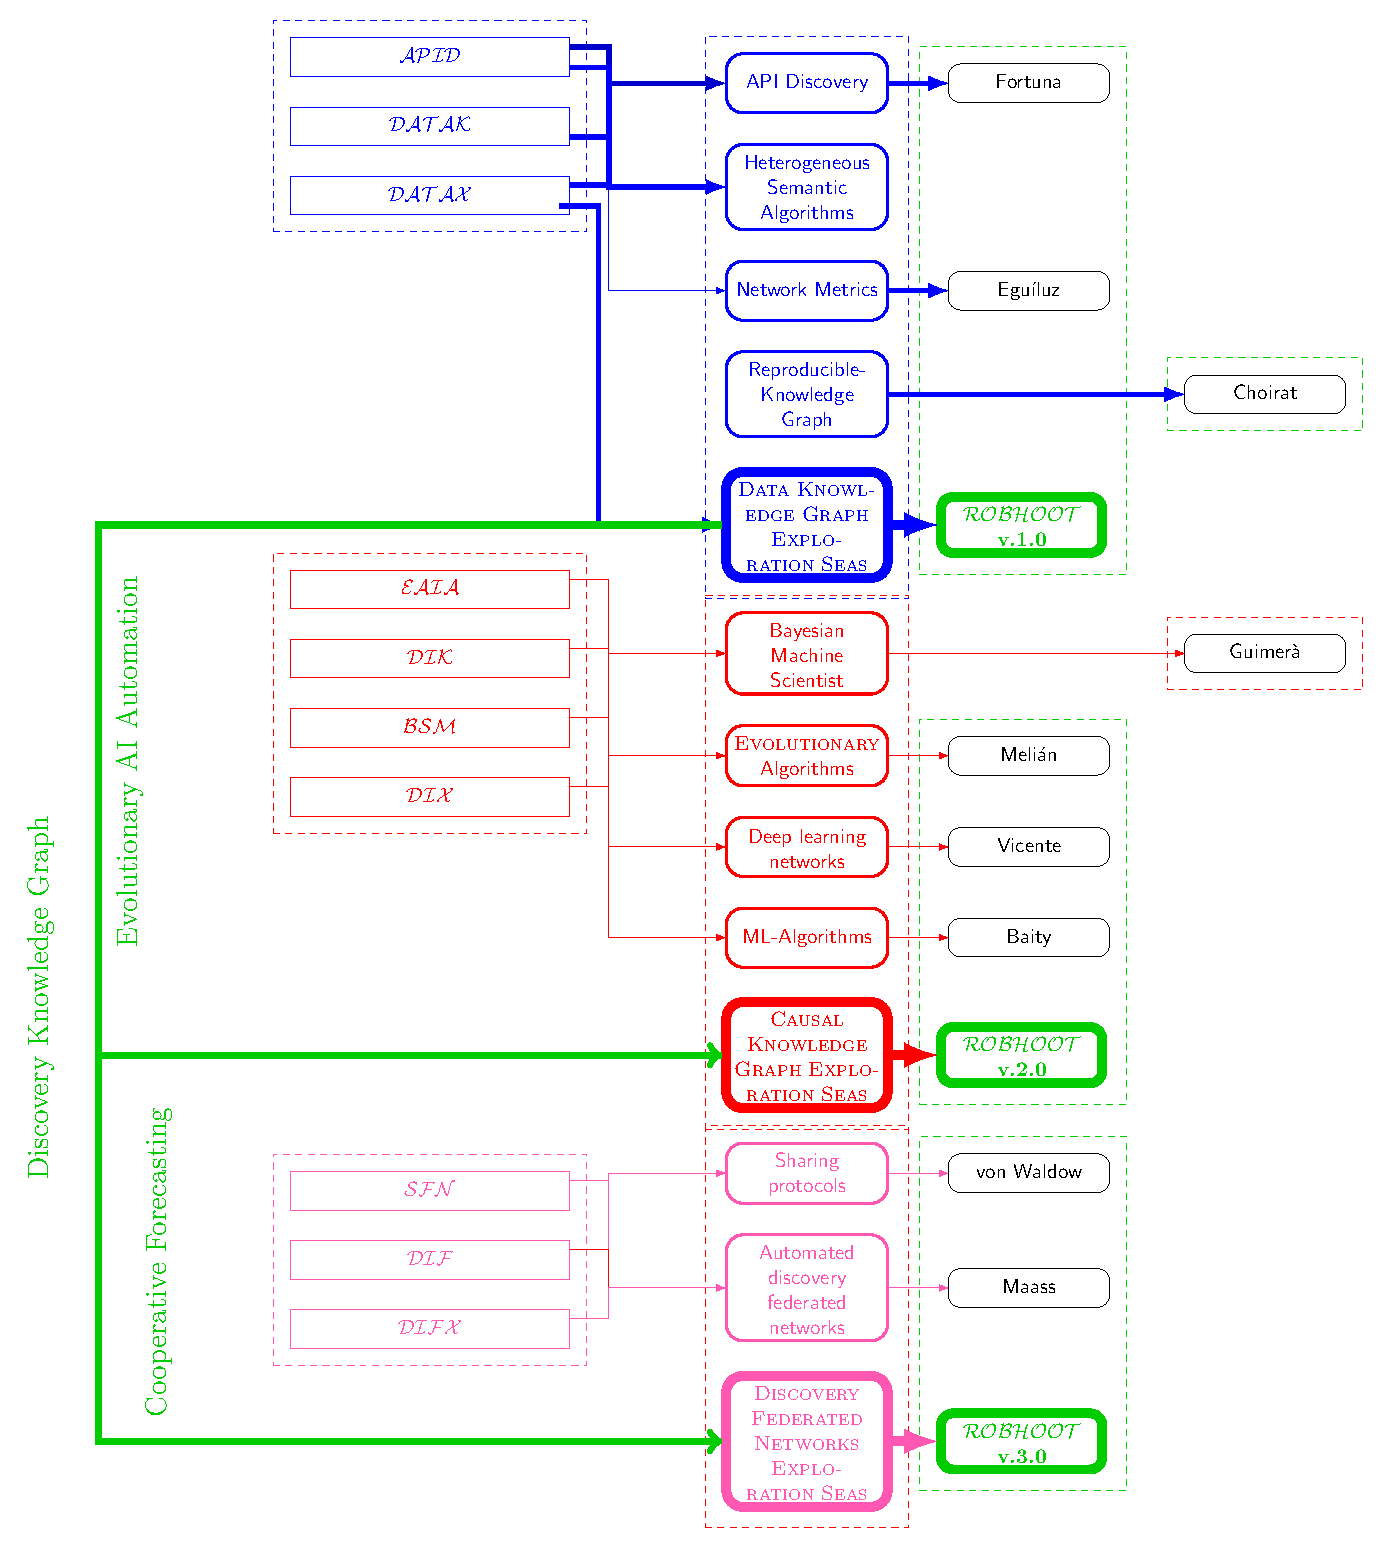
\includegraphics[width=12cm,height=22cm]{Figures/Consortium.pdf}}
\end{figure}
  
  
  \subsection{Resources to be committed}
 
  \begin{itemize}
  \item \textcolor{red}{Please make sure the information in this
      section matches the costs as stated in the budget table in
      section 3 of the administrative proposal forms, and the number
      of person months, shown in the detailed work package
      descriptions.  Please provide the following:}
 \item \textcolor{red}{a table showing number of person months required
    (table 3.4a)}
  \item \textcolor{red}{a table showing ‘other direct costs’ (table
      3.4b) for participants where those costs exceed 15\% of the
      personnel costs (according to the budget table in section 3 of
      the administrative proposal forms)}
\end{itemize}

  

\newpage

\section{Members of the consortium}

\begin{comment}
 This section is not covered by the page limit.

 The information provided here will be used to judge the operational
 capacity. Please make sure that you do not include information here
 that relates to the headings under sections 1 to 3. Experts will be
 instructed to ignore any information here which appears to have been
 included to circumvent page limits applying to those sections.
 \end{comment}

 \subsection{Participants (applicants)}

 \begin{itemize}
 \item \textcolor{red}{For each participant, provide the following: a
     description of the legal entity and its main tasks, with an
     explanation of how its profile matches the tasks in the proposal}
 \item \textcolor{red}{a curriculum vitae or description of the
     profile of the persons, including their gender, who will be
     primarily responsible for carrying out the proposed research
     and/or innovation activities. Indicate each person who would be a
     first-time participant to FET under Horizon 2020}
\item \textcolor{red}{a list of up to 5 relevant publications, and/or
    products, services (including widely-used datasets or software),
    or other achievements relevant to the call content}
\item \textcolor{red}{List of up to 5 relevant previous projects or
    activities, connected to the subject of this proposal}
 \item \textcolor{red}{a description of any significant infrastructure
     and/or any major items of technical equipment, relevant to the
     proposed work}
 \item \textcolor{red}{if operational capacity cannot be demonstrated
     at the time of submitting the proposal, describe the concrete
     measures that will be taken to obtain it by the time of the
     implementation of the task}
 \end{itemize}


 \begin{itemize}
 \item (description legal identity) Dr. Carlos Meli\'an is a tenured
   researcher in Theoretical Evolutionary Ecology at EAWAG, ETH-Domain
   in Switzerland, and associate professor at the University of Bern.
       (CV, gender, responsible research proposed, first time participant FET)

       He is the principal coordinator of the proposal.  Dr. Meli\'an
       has broad expertise in evolutionary algorithms and
       eco-evolutionary dynamics in ecological communities and
       biodiversity.
  
       (5 pubs)
       • Melián C, et al. 2018. Deciphering the interdependence
       between ecological and evolutionary networks. Trends in ecology
       & evolution 33,7: 504-512.  • Andreazzi C, Guimaraes P, Melián
       C. 2018. Eco-evolutionary feedbacks promote fluctuating
       selection and long-term stability of antagonistic
       networks. Proc. R. Soc. B 285: 20172596.  • Melián C, Seehausen
       O, Eguiluz V, Fortuna M, Deiner K. 2015. Diversification and
       Biodiversity Dynamics of Hot and Cold Spots. Ecography 38,
       393-401.  • Melián C, et al. 2015. Dispersal dynamics in food
       webs. American Naturalist 185, 2: 157-168.  • Melián C., et
       al. 2014. Individual trait variation and diversity in food
       webs. Advances in Ecological Research. Vol. 50. Academic Press,
       207-241.



 \item {\bf Victor M. Egu\'iluz (IFISC, CSIC, Spain)}: IFISC is an
   Maria de Maetzu Excellent center at the UIB, Balearic
   Islands. Dr. Egu\'iluz has expertise in health-related topics, in
   particular he has developed collaborations with Harvard medical
   school and many biodiversity and sustainability research
   institutions. The group of the PL has worked in the development of
   data-driven agent-based networks in social, biological and
   environmental problems with particular relevance in epidemiological
   networks.
\item
\item
   \end{itemize}

 
 \subsection{Third parties involved in the project (including use of third party resources)}


\begin{itemize}
\item \textcolor{red}{For each participant, does the participant plan
    to subcontract certain tasks (please note that core tasks of the
    project should not be sub-contracted) Y/N If yes, please describe
    and justify the tasks to be subcontracted}
\item \textcolor{red}{Does the participant envisage that part of its
    work is performed by linked third parties2 Y/N If yes, please
    describe the third party, the link of the participant to the third
    party, and describe and justify the foreseen tasks to be performed
    by the third party}
\item \textcolor{red}{Does the participant envisage the use of
    contributions in kind provided by third parties (Articles 11 and
    12 of the General Model Grant Agreement) Y/N If yes, please
    describe the third party and their contributions}
\item \textcolor{red}{Does the participant envisage that part of the
    work is performed by International Partners3 (Article 14a of the
    General Model Grant Agreement)?  Y/N If yes, please describe the
    International Partner(s) and their contributions.}
\end{itemize}


\section{Ethics and Security}

 This section is not covered by the page limit.

\subsection{Ethics}


\textcolor{red}{ For more guidance, see the document "How to complete
  your ethics self-assessment".  If you have entered any ethics issues
  in the ethical issue table in the administrative proposal forms, you
  must:}

\begin{itemize}
\item \textcolor{red}{submit an ethics self-assessment, which:}
\item \textcolor{red}{describes how the proposal meets the national
    legal and ethical requirements of the country or countries where
    the tasks raising ethical issues are to be carried out;}
\item \textcolor{red}{explains in detail how you intend to address the
    issues in the ethical issues table, in particular as regards:
    research objectives (e.g. study of vulnerable populations, dual
    use, etc.)  ▪ research methodology (e.g. clinical trials,
    involvement of children and related consent procedures, protection
    of any data collected, etc.)}
\item \textcolor{red}{the potential impact of the research (e.g. dual
    use issues, environmental damage, stigmatisation of particular
    social groups, political or financial retaliation,
    benefit-sharing, misuse, etc.)}
\item \textcolor{red}{provide the documents that you need under
    national law(if you already have them), e.g.: ◦ an ethics
    committee opinion; ◦ the document notifying activities raising
    ethical issues or authorising such activities If these documents
    are not in English, you must also submit an English summary of
    them (containing, if available, the conclusions of the committee
    or authority concerned).

    \\
    If you plan to request these documents specifically for the project
  you are proposing, your request must contain an explicit reference
  to the project title.}

\subsection{Security}


\textcolor{red{Please indicate if your project will involve:}

\begin{itemize}
\item \textcolor{red}{activities or results raising security issues:
    (YES/NO)}
\item \textcolor{red}{EU-classified information as background or
    results: (YES/NO)}
\end{itemize}  



%----------------------------------------------------------------------------------------
%	BIBLIOGRAPHY
%----------------------------------------------------------------------------------------

%\printbibliography[title={Bibliography}] % Print the bibliography, section title in curly brackets

\newpage
\bibliographystyle{unsrtnat}
%\bibliographystyle{tree.bst}
\bibliography{Robhoot.bib}

%----------------------------------------------------------------------------------------

\end{document}
